%% Ein einfaches Template für einen Übungsbericht unter Verwendung des Hagenberg
%% Setups, basierend auf der LaTeX 'report' Standardklasse.
%%% äöüÄÖÜß  <-- keine deutschen Umlaute hier? UTF-faehigen Editor verwenden!

%%% Magic Comments zum Setzen der korrekten Parameter in kompatiblen IDEs
% !TeX encoding = utf8
% !TeX program = pdflatex
% !TeX spellcheck = de_DE
% !BIB program = biber

\documentclass[german,notitlepage,smartquotes]{hgbreport}
% Zulässige Optionen in [..]:
%    Hauptsprache: 'german' (default), 'english'
%    Option zur Umwandlung in typografische Anführungszeichen: 'smartquotes'
%    APA Zitierstil: 'apa'
%    Erzeuge keine separate Titelseite: 'notitlepage'
%%%-----------------------------------------------------------------------------

\RequirePackage[utf8]{inputenc} % bei Verw. von lualatex oder xelatex entfernen!

\renewcommand{\chapter}[1]{} % Deaktiviere den \chapter Befehl
\graphicspath{{images/}}     % Verzeichnis mit Bildern und Grafiken
\bibliography{references}    % Biblatex-Literaturdatei (references.bib)
\ExecuteBibliographyOptions{backref=false} % Keine Rückreferenzen bei Quellen

%%%-----------------------------------------------------------------------------
\setcounter{chapter}{4}	% <----- Auf die Übungsnummer setzen
%%%-----------------------------------------------------------------------------

\author{Julian Jany}                        % Name
\title{GP2 Generative Programmierung -- SS 2022\\ % Name der Übung
				Übungsabgabe \arabic{chapter}}
\date{\today}

%%%-----------------------------------------------------------------------------
\begin{document}
%%%-----------------------------------------------------------------------------
\maketitle
%%%-----------------------------------------------------------------------------

\lstset{language=Java,
		basicstyle=\ttfamily\footnotesize,
		keywordstyle=\color{blue}\ttfamily,
		stringstyle=\color{red}\ttfamily,
		commentstyle=\color[rgb]{0,0.608,0.333}\ttfamily, % ForestGreen
		morecomment=[l][\color{magenta}]{\#}
}

%%%-----------------------------------------------------------------------------

\section{Tracing}

\subsection{Lösungsidee}

Gemeinsam in der Übung implementiert.

\subsection{Code}

\lstinputlisting[caption=Tracing.aj, language={Java}]{src/Tracing/src/main/java/aspects/Tracing.aj}
\lstinputlisting[caption=Indentation.aj, language={Java}]{src/Tracing/src/main/java/aspects/Indentation.aj}
\lstinputlisting[caption=PositiveValues.java, language={Java}]{src/Tracing/src/main/java/application/PositiveValues.java}
\lstinputlisting[caption=Main.java, language={Java}]{src/Tracing/src/main/java/application/Main.java}

\clearpage

\subsection{Test}

\begin{figure}[h]
\centering
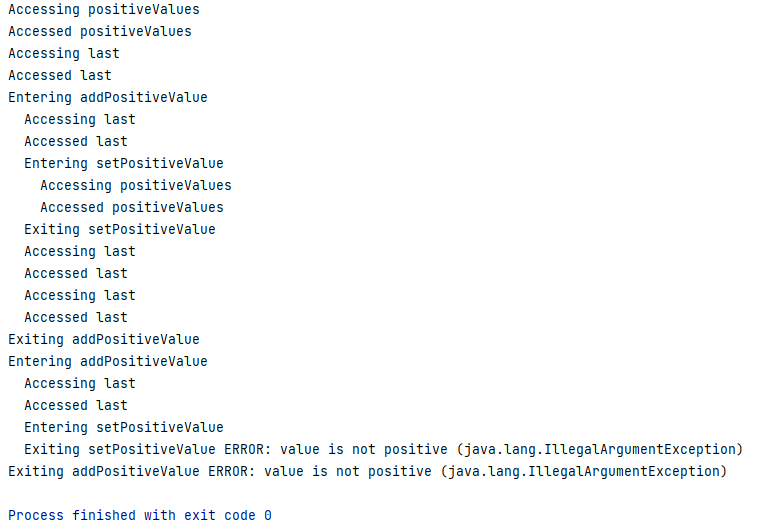
\includegraphics[width=.7\textwidth]{tracing-test-0}
\caption{Testausgabe des Tracing Projekts}
\label{fig:tracing-test-0}
\end{figure}

%%%-----------------------------------------------------------------------------

\clearpage

\section{Caching}

\subsection{Lösungsidee}

Alles bis auf den Aspekt \texttt{RuntimeMeasurement} wurde gemeinsam in der Übung implementiert.

Bei der Umsetzung war zu beachten, dass -- wie schon bei \texttt{LogRecursiveCalls} -- nur der äußerste Aufruf von \texttt{BinomialCoefficient.calculate(...)} zum Pointcut gehört. Zudem wurde die Priorität so festgelegt, dass \texttt{RuntimeMeasurement} die niedrigste Priorität aufweist. Das bewirkt, dass nur die Laufzeit der Berechnung gemessen wird -- exklusive möglicher zusätzlicher Advices.

\subsection{Code}

\lstinputlisting[caption=BinomialCache.aj, language={Java}]{src/Caching/src/main/java/aspects/BinomialCache.aj}
\lstinputlisting[caption=LogRecursiveCalls.aj, language={Java}]{src/Caching/src/main/java/aspects/LogRecursiveCalls.aj}
\lstinputlisting[caption=RuntimeMeasurement.aj, language={Java}]{src/Caching/src/main/java/aspects/RuntimeMeasurement.aj}
\lstinputlisting[caption=BinomialCoefficient.java, language={Java}]{src/Caching/src/main/java/application/BinomialCoefficient.java}
\lstinputlisting[caption=Caching.java, language={Java}]{src/Caching/src/main/java/application/Caching.java}

\clearpage

\subsection{Test}

\begin{figure}[h]
\centering
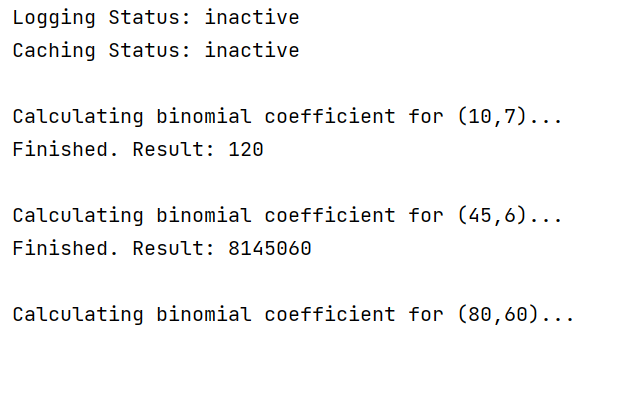
\includegraphics[width=.5\textwidth]{caching-test-00}
\caption{Ausgabe Caching; Alle Advices deaktiviert}
\label{caching-test-00}
\end{figure}

\begin{figure}[h]
\centering
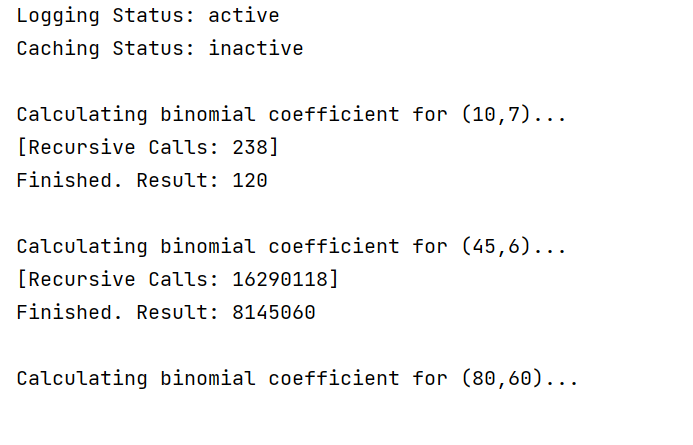
\includegraphics[width=.5\textwidth]{caching-test-01}
\caption{Ausgabe Caching; \texttt{loggingEnabled}}
\label{caching-test-01}
\end{figure}

\begin{figure}[h]
\centering
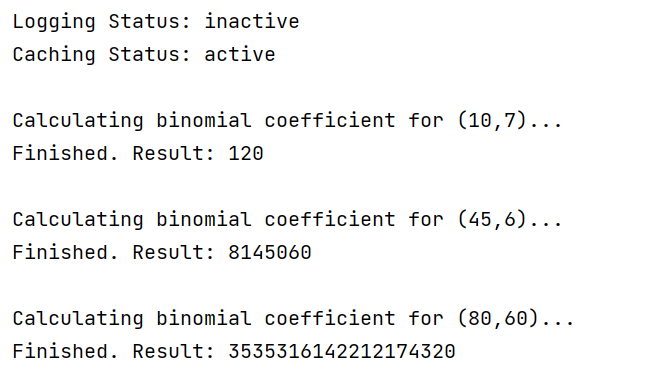
\includegraphics[width=.5\textwidth]{caching-test-02}
\caption{Ausgabe Caching; \texttt{cachingEnabled}}
\label{caching-test-02}
\end{figure}

\begin{figure}[h]
\centering
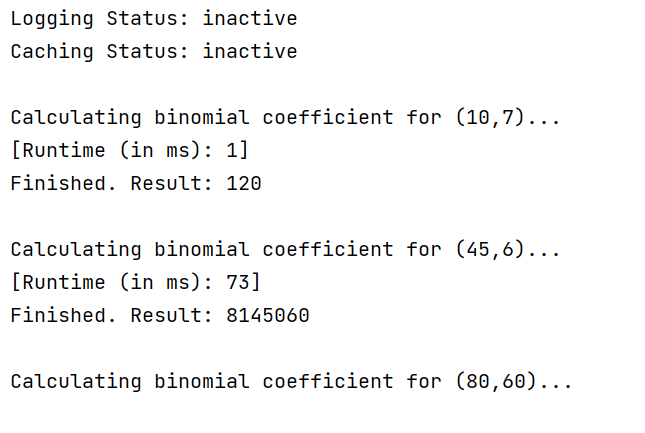
\includegraphics[width=.5\textwidth]{caching-test-03}
\caption{Ausgabe Caching; \texttt{runtimeMeasurementEnabled}}
\label{caching-test-03}
\end{figure}

\begin{figure}[h]
\centering
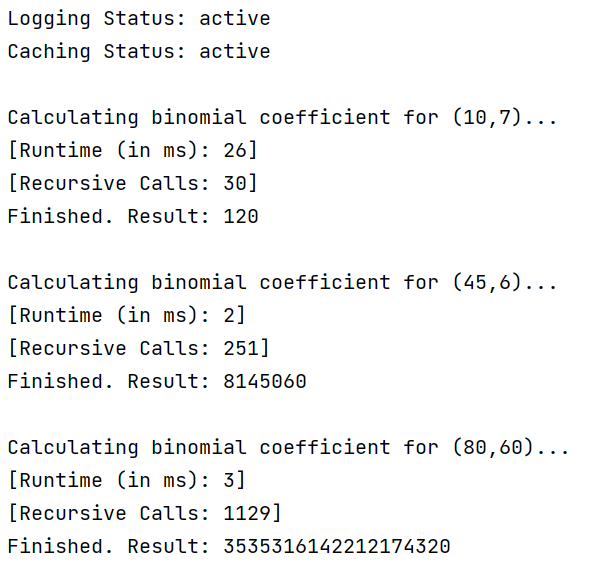
\includegraphics[width=.5\textwidth]{caching-test-04}
\caption{Ausgabe Caching; Alle Advices aktiviert}
\label{caching-test-04}
\end{figure}

%%%-----------------------------------------------------------------------------

\clearpage

\section{Aspect-Oriented TSP Solver}

\subsection{Lösungsidee}

\subsubsection{CountEvaluatedSolutions}

Nach jedem Aufruf von \texttt{Solution.evaluate()} wird eine interne Zählvariable inkrementiert. Nach jedem Aufruf von \texttt{Algorithm.execute()} wird dieser Zähler ausgegeben und zurückgesetzt.

\subsubsection{LimitEvaluatedSolutions}

Dieser Aspekt erweitert den Aspekt \texttt{CountEvaluatedSolutions}. Der Zähler des Basis-Aspekts wird verwendet um das Abbruchkriterium des Algorithmus zu verändern. Es wird ein Around-Advice implementiert welcher das Ergebnis von \texttt{Algorithm.isTer\-mi\-na\-ted()} verändert; \texttt{Algorithm.isTerminated()} soll \texttt{true} liefern, wenn der Rückgabewert des tatsächlichen Aufrufs \texttt{true} liefert (inklusiv-) oder die Maximalanzahl an Evaluierungen erreicht ist. Der Algorithmus wird also nicht sofort abgebrochen, wenn die Maximalanzahl an Evaluierungen erreicht wurde, sondern es werden -- wie in der Angabe gefordert -- die Evaluierungen der aktuellen Iteration abgeschlossen.

\subsubsection{Elitism}

Es wird ein Around-Advice implementiert welcher den Übergabe-Parameter -- \texttt{Solu\-tion[] children} -- an \texttt{GA.replace(..)} verändert. Die schlechteste Solution der neuen Population wird durch die aktuell beste Solution ersetzt.

\subsubsection{ProtocolProgress}

Es werden zwei Advices implementiert; einer welcher nach jedem Aufruf von \texttt{Algorithm\-.\-initialize()} oder \texttt{Algorithm.iterate()} Statistiken über die aktuelle Population sammelt und ein weiterer welcher nach jedem Aufruf von \texttt{Algorithm.execute()} die gesammelten Statistiken in verschiedenen Formen ausgibt/visualisiert und danach die Collection der Statistiken leert. Bei der Implementierung ist zu beachten, dass innerhalb der Advices der Zugriff auf den \texttt{GA} bzw. die \texttt{population} möglich sein muss. Eine Möglichkeit das umzusetzen ist, bei den entsprechenden Pointcuts \texttt{target(ga)} anzugeben. Falls Zugriff auf private Member/Methoden benötigt wird, muss der Aspekt als \texttt{privileged} deklariert werden.

\subsection{Code}

\lstinputlisting[caption=Pointcuts.aj, language={Java}]{src/TSP/src/main/java/aspects/Pointcuts.aj}
\lstinputlisting[caption=CountEvaluatedSolutions.aj, language={Java}]{src/TSP/src/main/java/aspects/CountEvaluatedSolutions.aj}
\lstinputlisting[caption=LimitEvaluatedSolutions.aj, language={Java}]{src/TSP/src/main/java/aspects/LimitEvaluatedSolutions.aj}
\lstinputlisting[caption=Elitism.aj, language={Java}]{src/TSP/src/main/java/aspects/Elitism.aj}
\lstinputlisting[caption=ProtocolProgress.aj, language={Java}]{src/TSP/src/main/java/aspects/ProtocolProgress.aj}
\lstinputlisting[caption=TSPSolver.java, language={Java}]{src/TSP/src/main/java/tsp/TSPSolver.java}

\clearpage

\subsection{Test}

\subsubsection{Zeitmessung und Zählen von Evaluierungs-Aufrufen}

\begin{figure}[h]
\centering
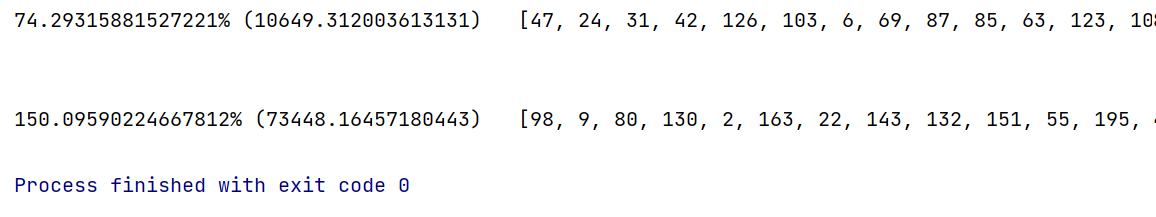
\includegraphics[width=.9\textwidth]{tsp-test-00}
\caption{Ausgabe TSP-Solver; Alle Advices deaktiviert}
\label{tsp-test-00}
\end{figure}

\begin{figure}[h]
\centering
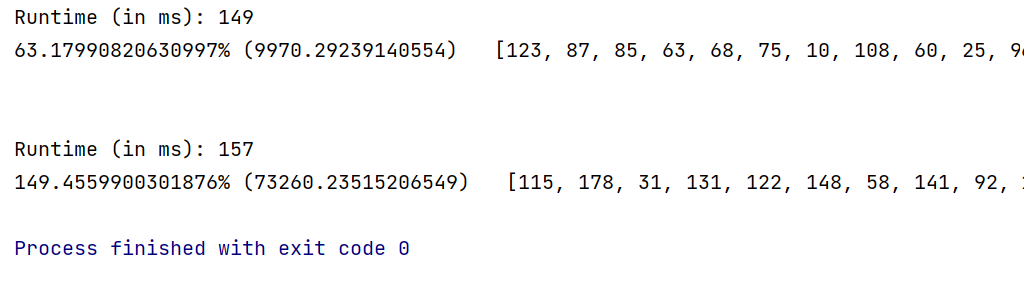
\includegraphics[width=.9\textwidth]{tsp-test-01}
\caption{Ausgabe TSP-Solver; \texttt{MeasureRuntime} Advice aktiviert}
\label{tsp-test-01}
\end{figure}

\begin{figure}[h]
\centering
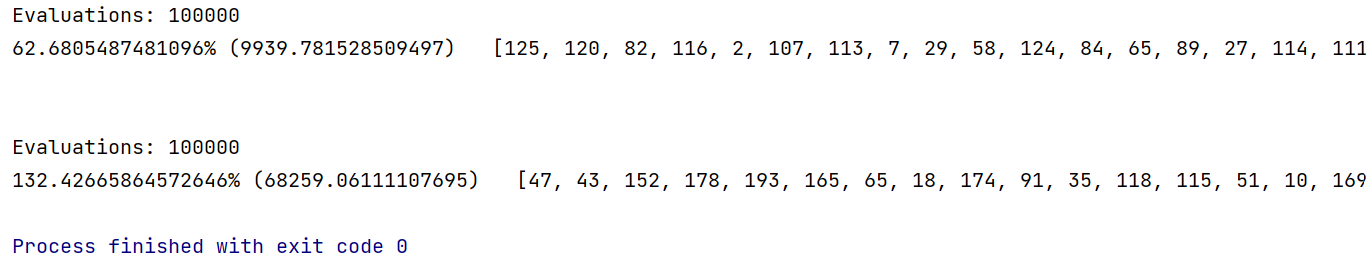
\includegraphics[width=.9\textwidth]{tsp-test-02}
\caption{Ausgabe TSP-Solver; \texttt{CountEvaluatedSolutions} Advice aktiviert}
\label{tsp-test-02}
\end{figure}

\begin{figure}[h]
\centering
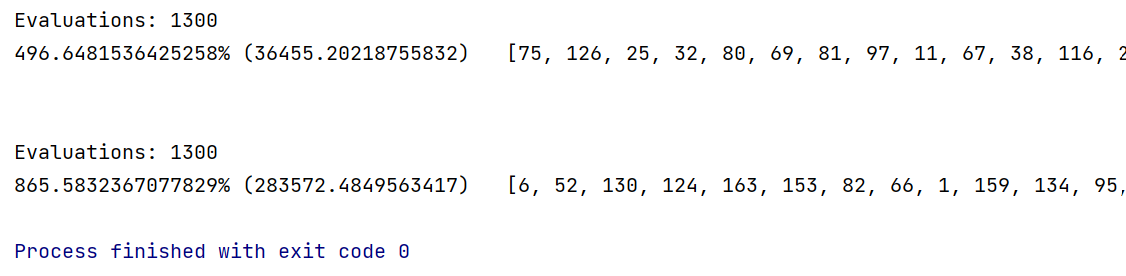
\includegraphics[width=.9\textwidth]{tsp-test-03}
\caption{Ausgabe TSP-Solver; \texttt{LimitEvaluatedSolutions} Advice ($maximumEvaluations=1234$) aktiviert}
\label{tsp-test-03}
\end{figure}

\begin{figure}[h]
\centering
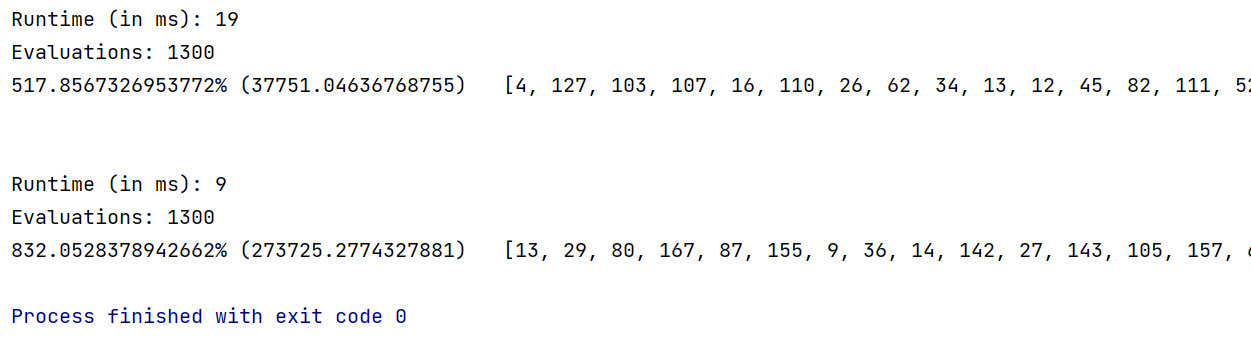
\includegraphics[width=.9\textwidth]{tsp-test-04}
\caption{Ausgabe TSP-Solver; \texttt{MeasureRuntime}, \texttt{CountEvaluatedSolutions} und \texttt{LimitEvaluatedSolutions} ($maximumEvaluations=1234$) Advices aktiviert}
\label{tsp-test-04}
\end{figure}

%----------------------------------------------------------------------------------------------------------------
\subsubsection{Aufzeichnen des Qualitätsverlaufs}

\begin{figure}[h]
\centering
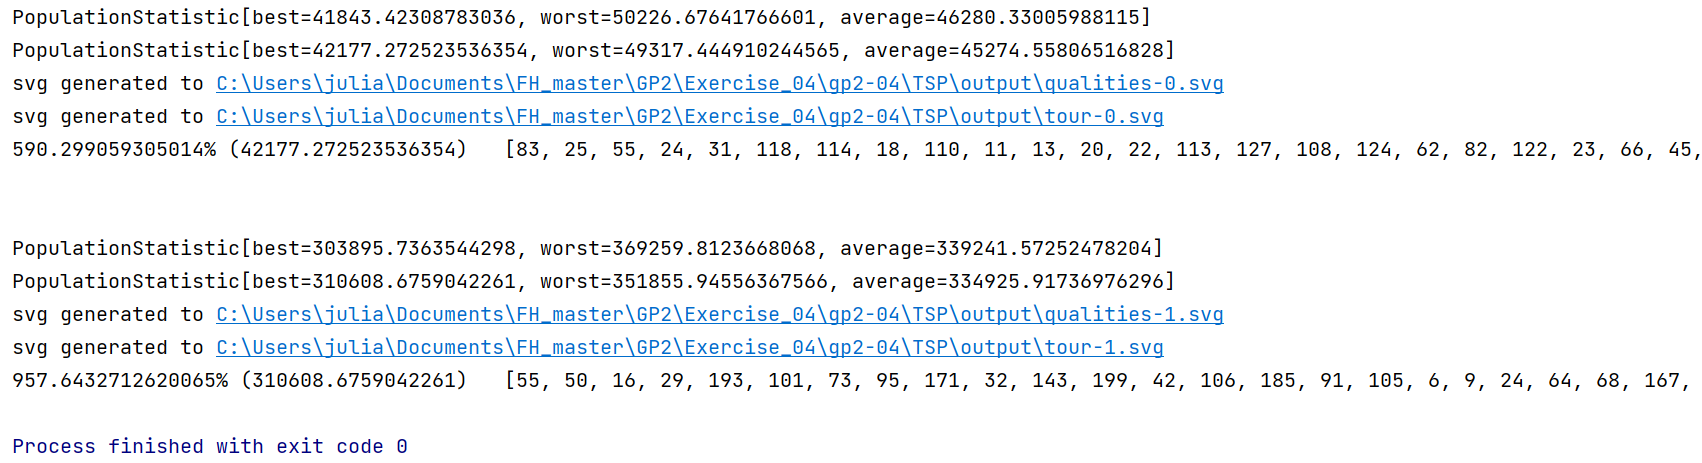
\includegraphics[width=.9\textwidth]{tsp-test-05}
\caption{Ausgabe TSP-Solver; \texttt{ProtocolProgress} Advices (Anzahl der Iterationen wurde auf $2$ gesetzt um die Ausgabe kurz zu halten) aktiviert}
\label{tsp-test-05}
\end{figure}

\begin{figure}[h]
\centering\small
\begin{tabular}{cc}
	\FramePic{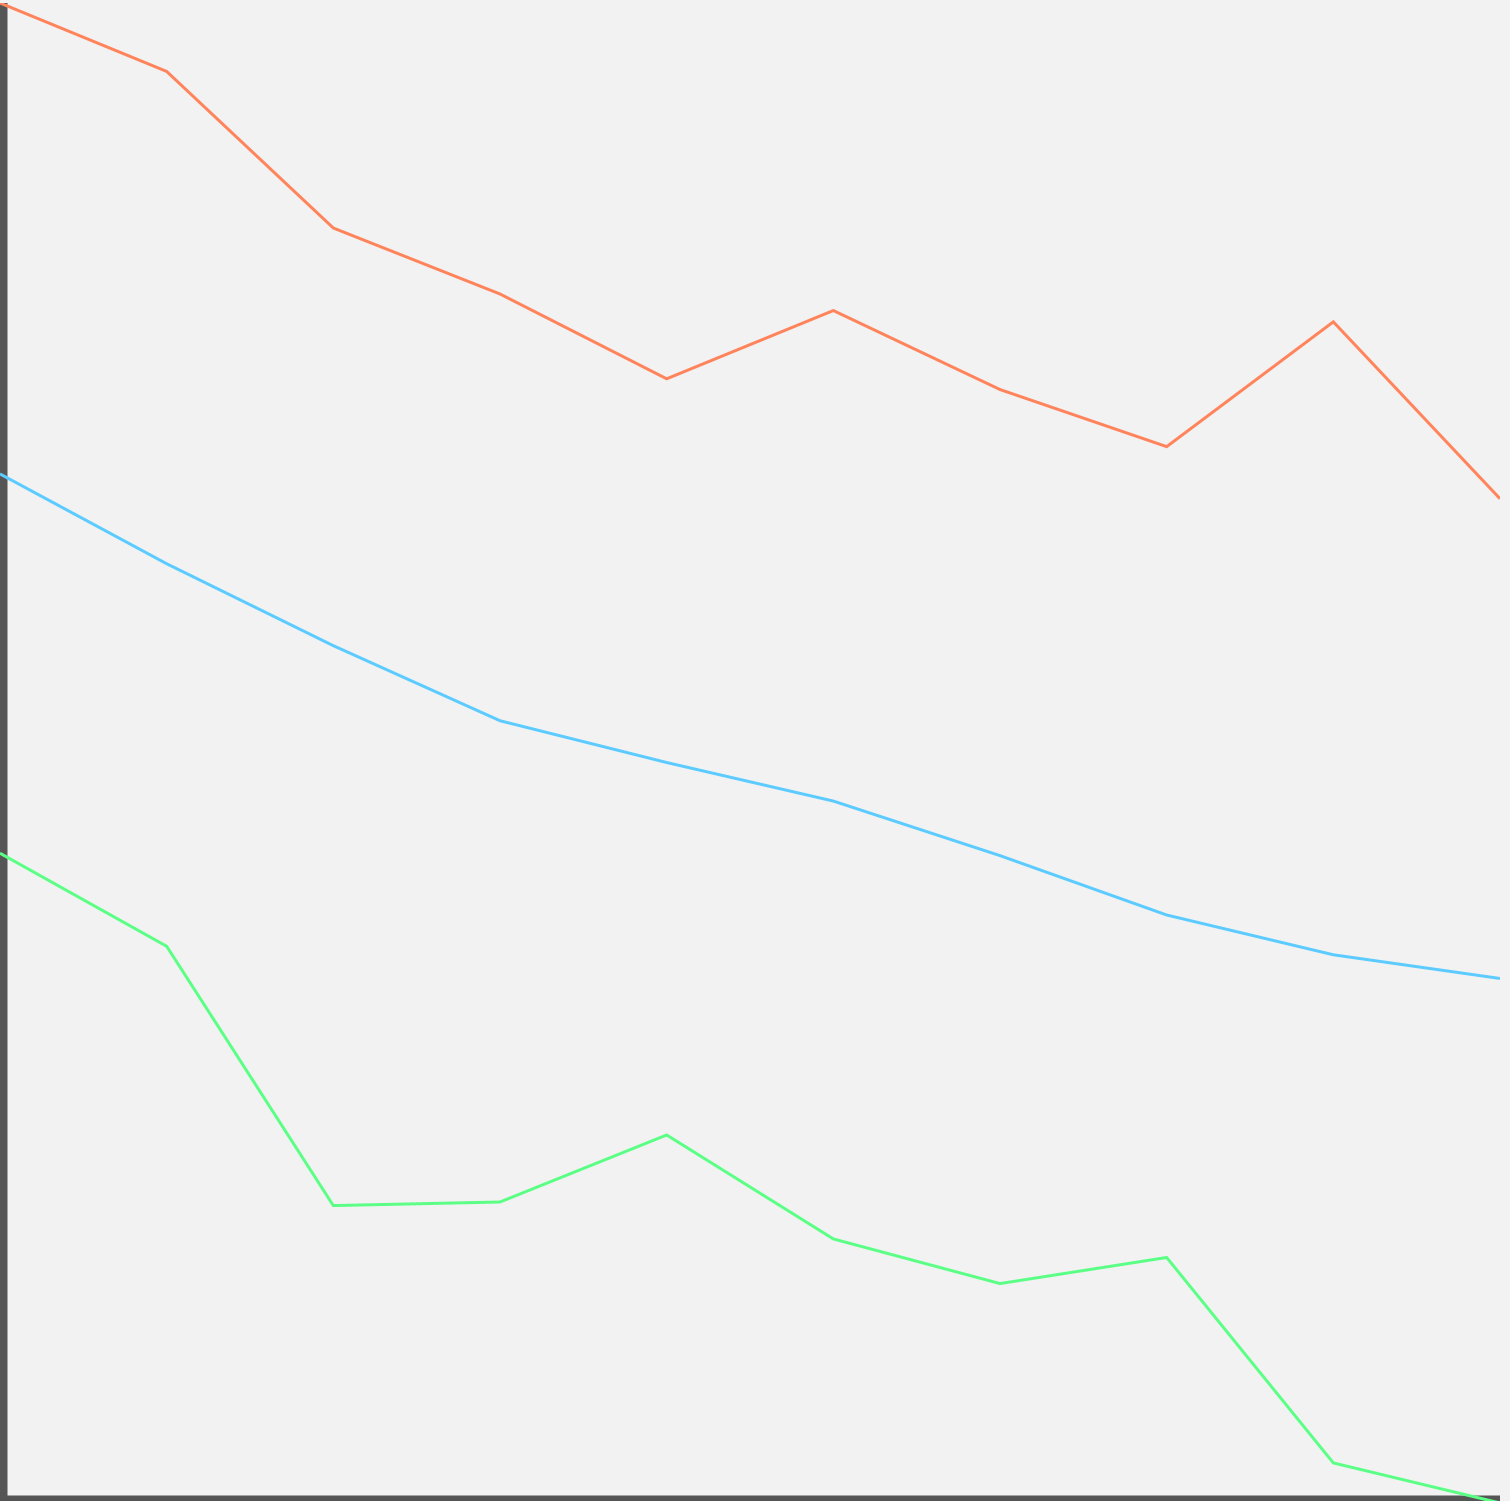
\includegraphics[width=0.45\textwidth]{tour-0-quality-10}} &
	\FramePic{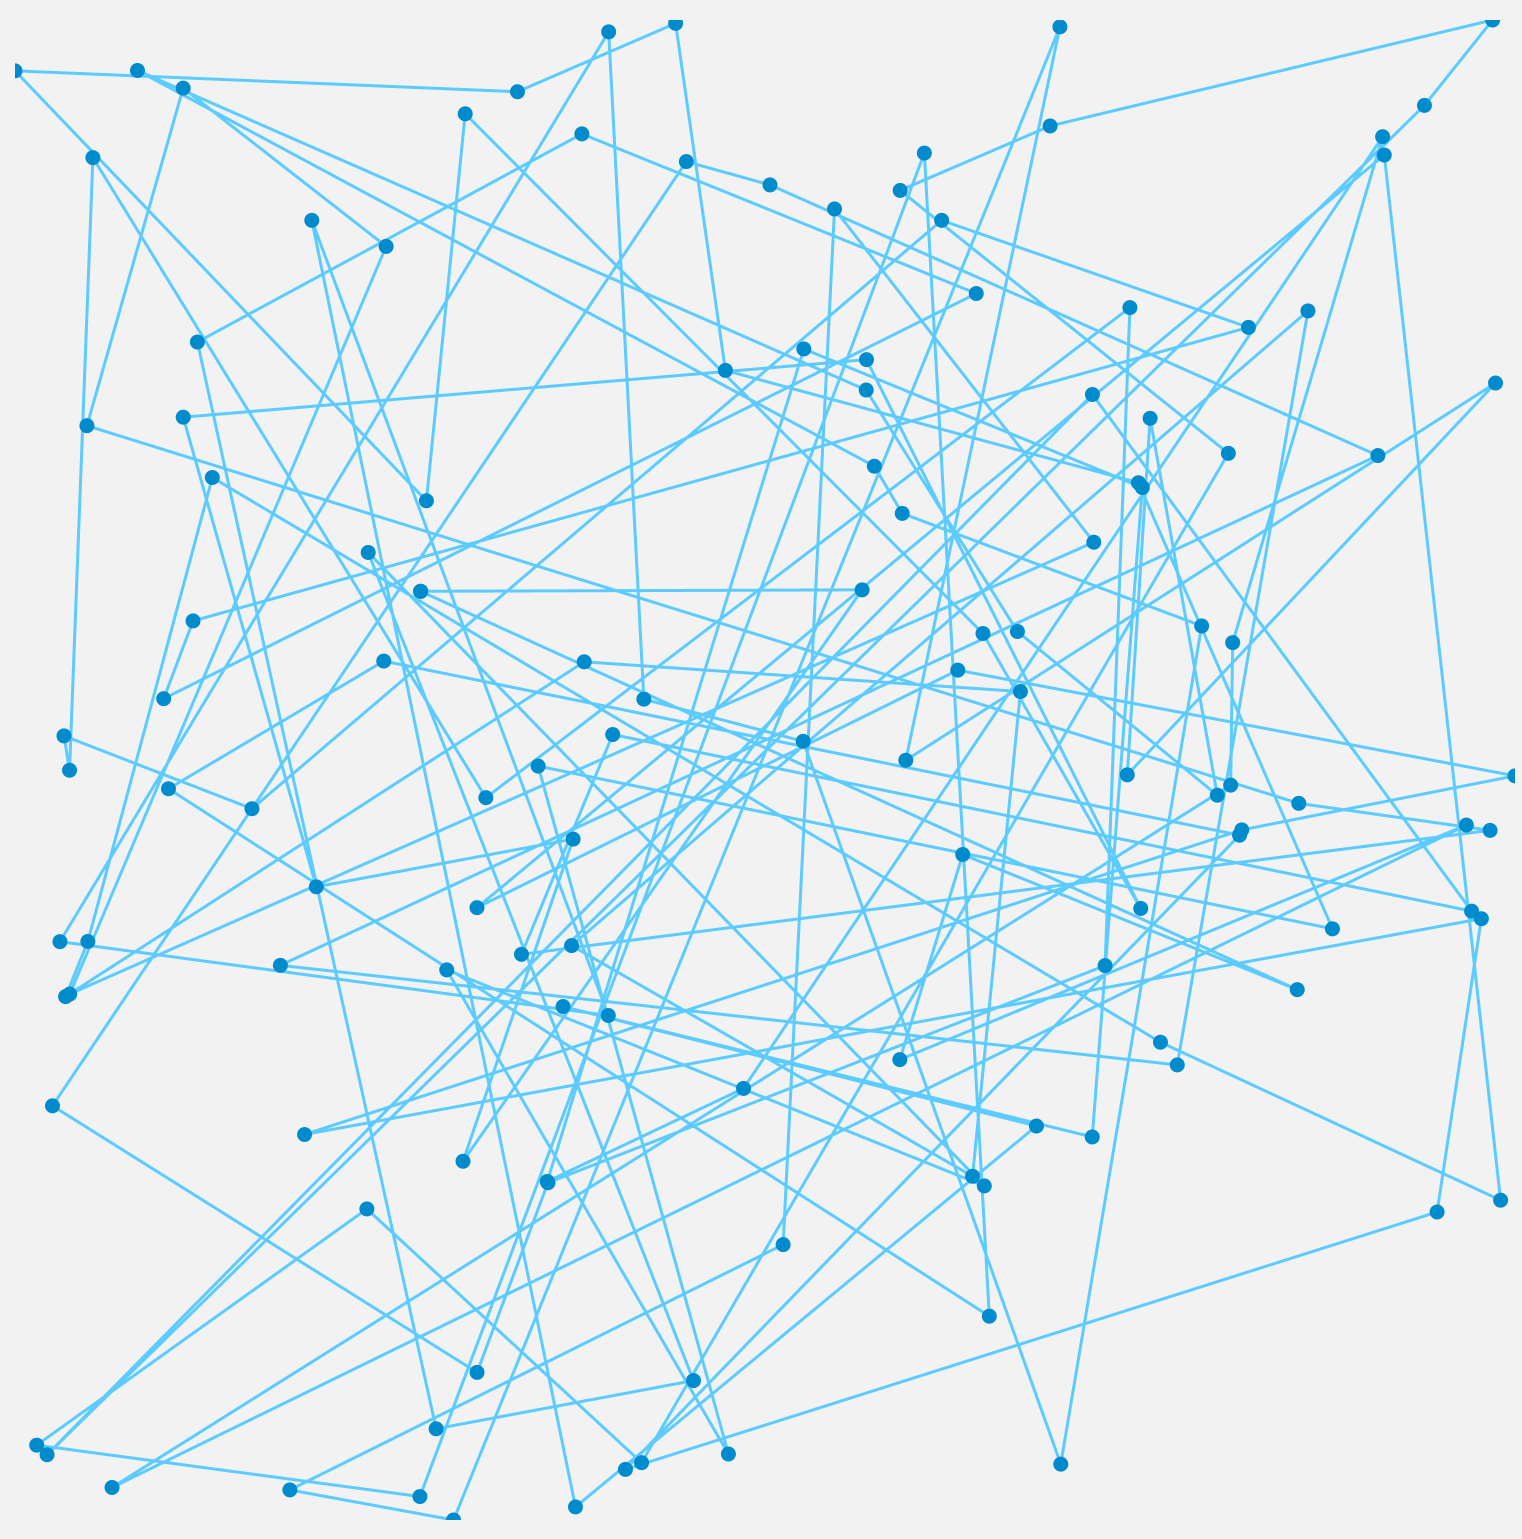
\includegraphics[width=0.45\textwidth]{tour-0-10}} \\
	(a) & (b) \\
	\FramePic{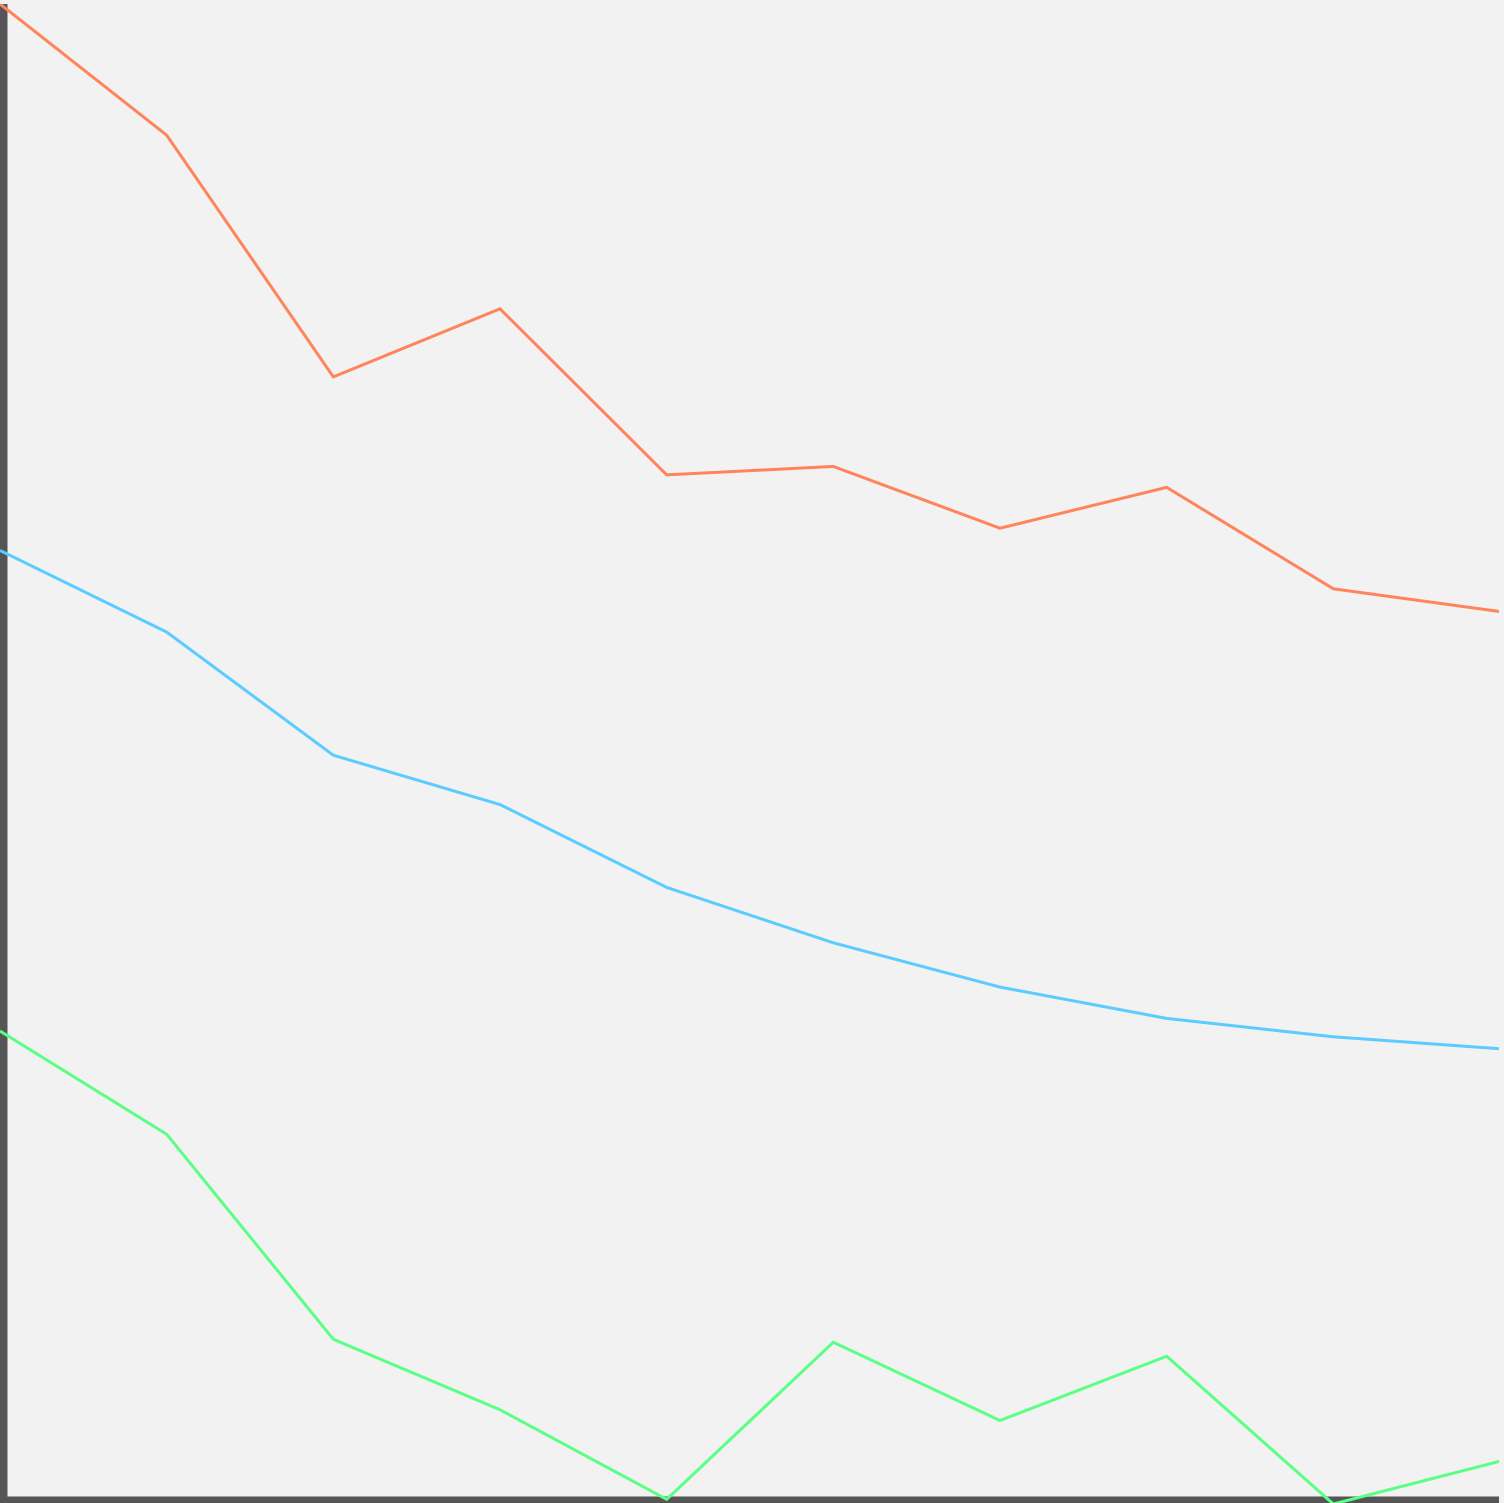
\includegraphics[width=0.45\textwidth]{tour-1-quality-10}} &
	\FramePic{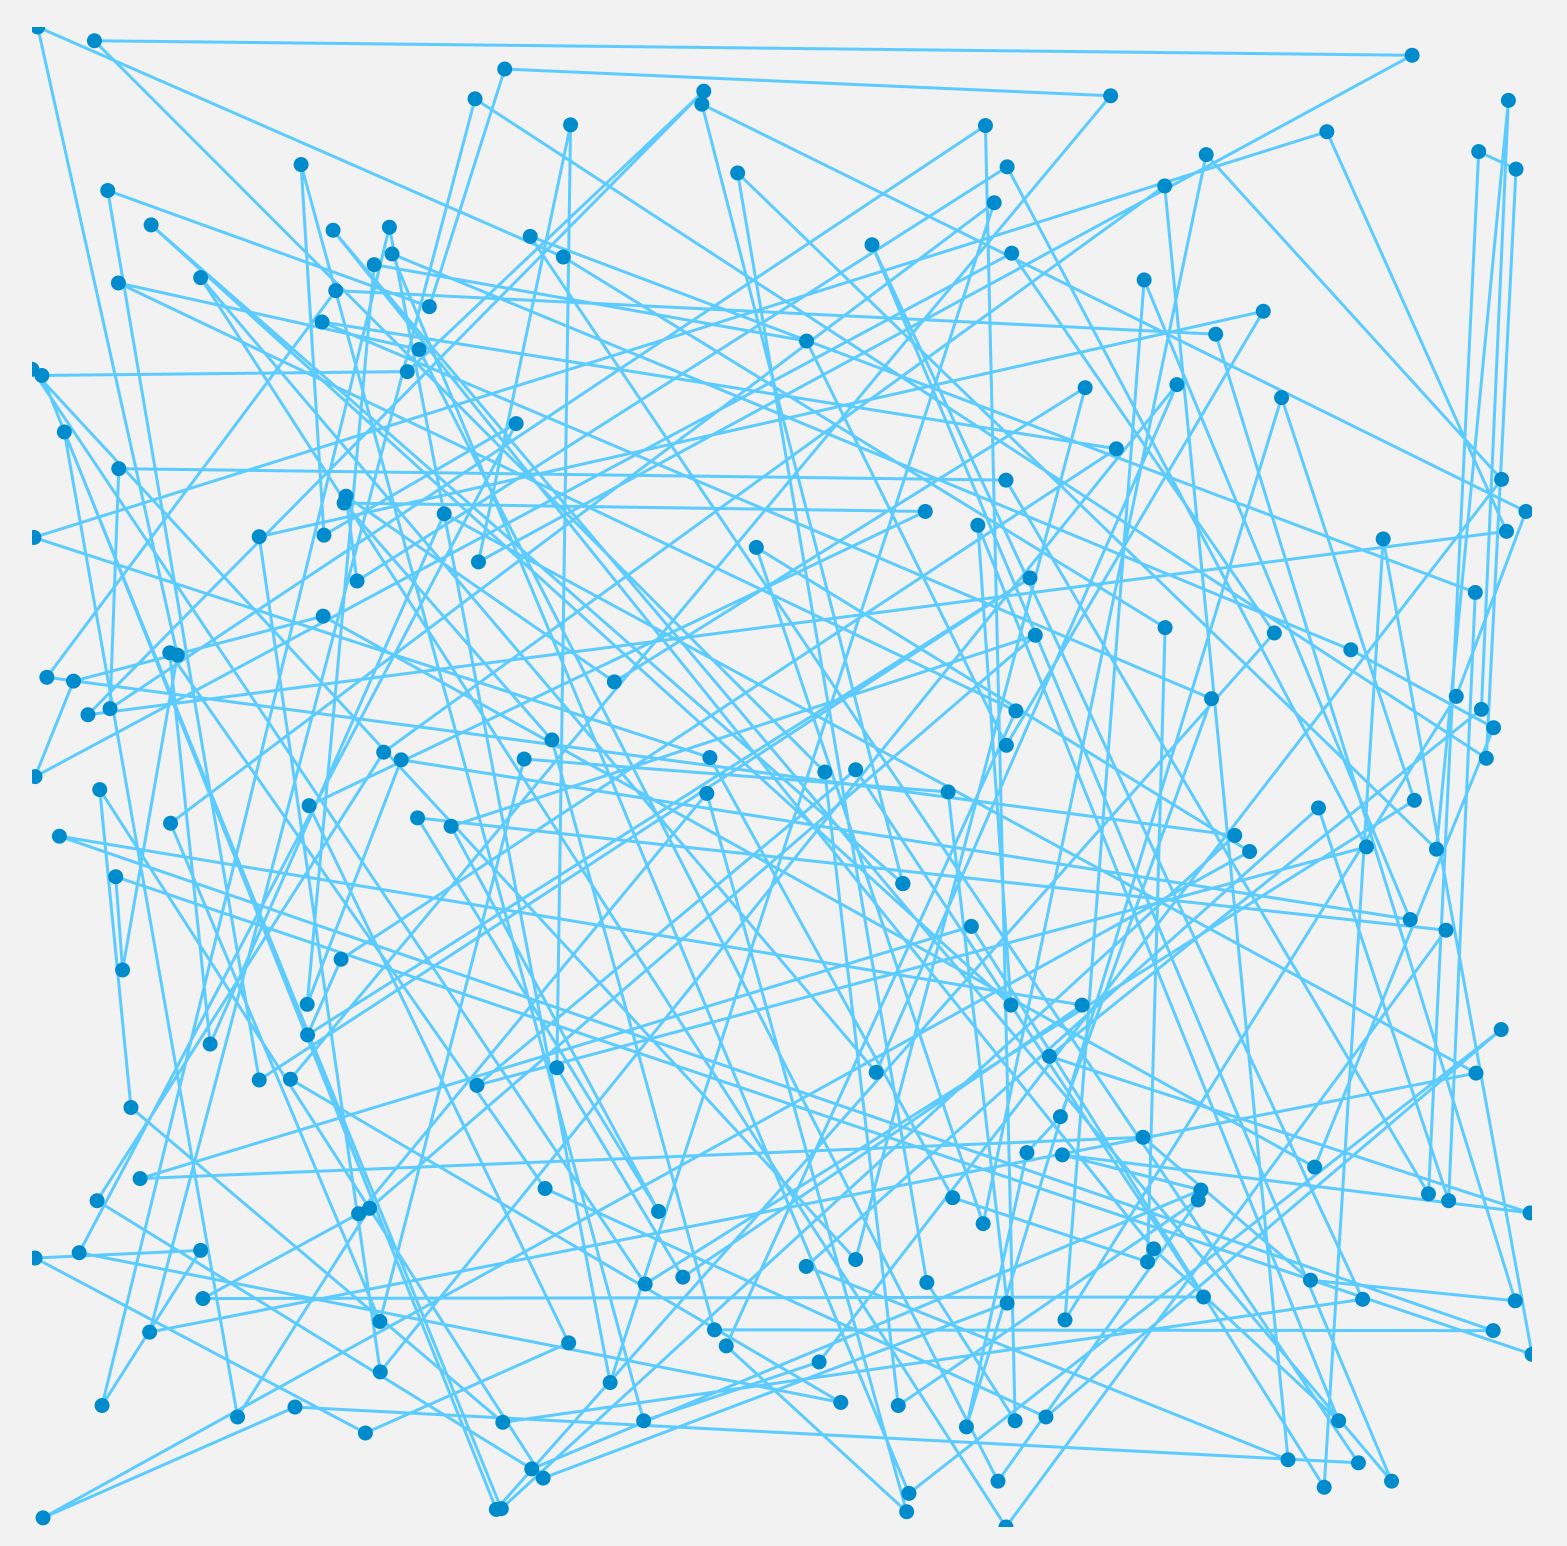
\includegraphics[width=0.45\textwidth]{tour-1-10}} \\
	(c) & (d)
\end{tabular}
\caption{Ergebnisse bei 10 Iterationen: 'ch130' Qualitätsverlauf~(a); 'ch130' beste Tour~(b); 'kroA200' Qualitätsverlauf~(c) 'kroA200' beste Tour~(d).}
\label{fig:tour-x-10}
\end{figure}

\begin{figure}[h]
\centering\small
\begin{tabular}{cc}
	\FramePic{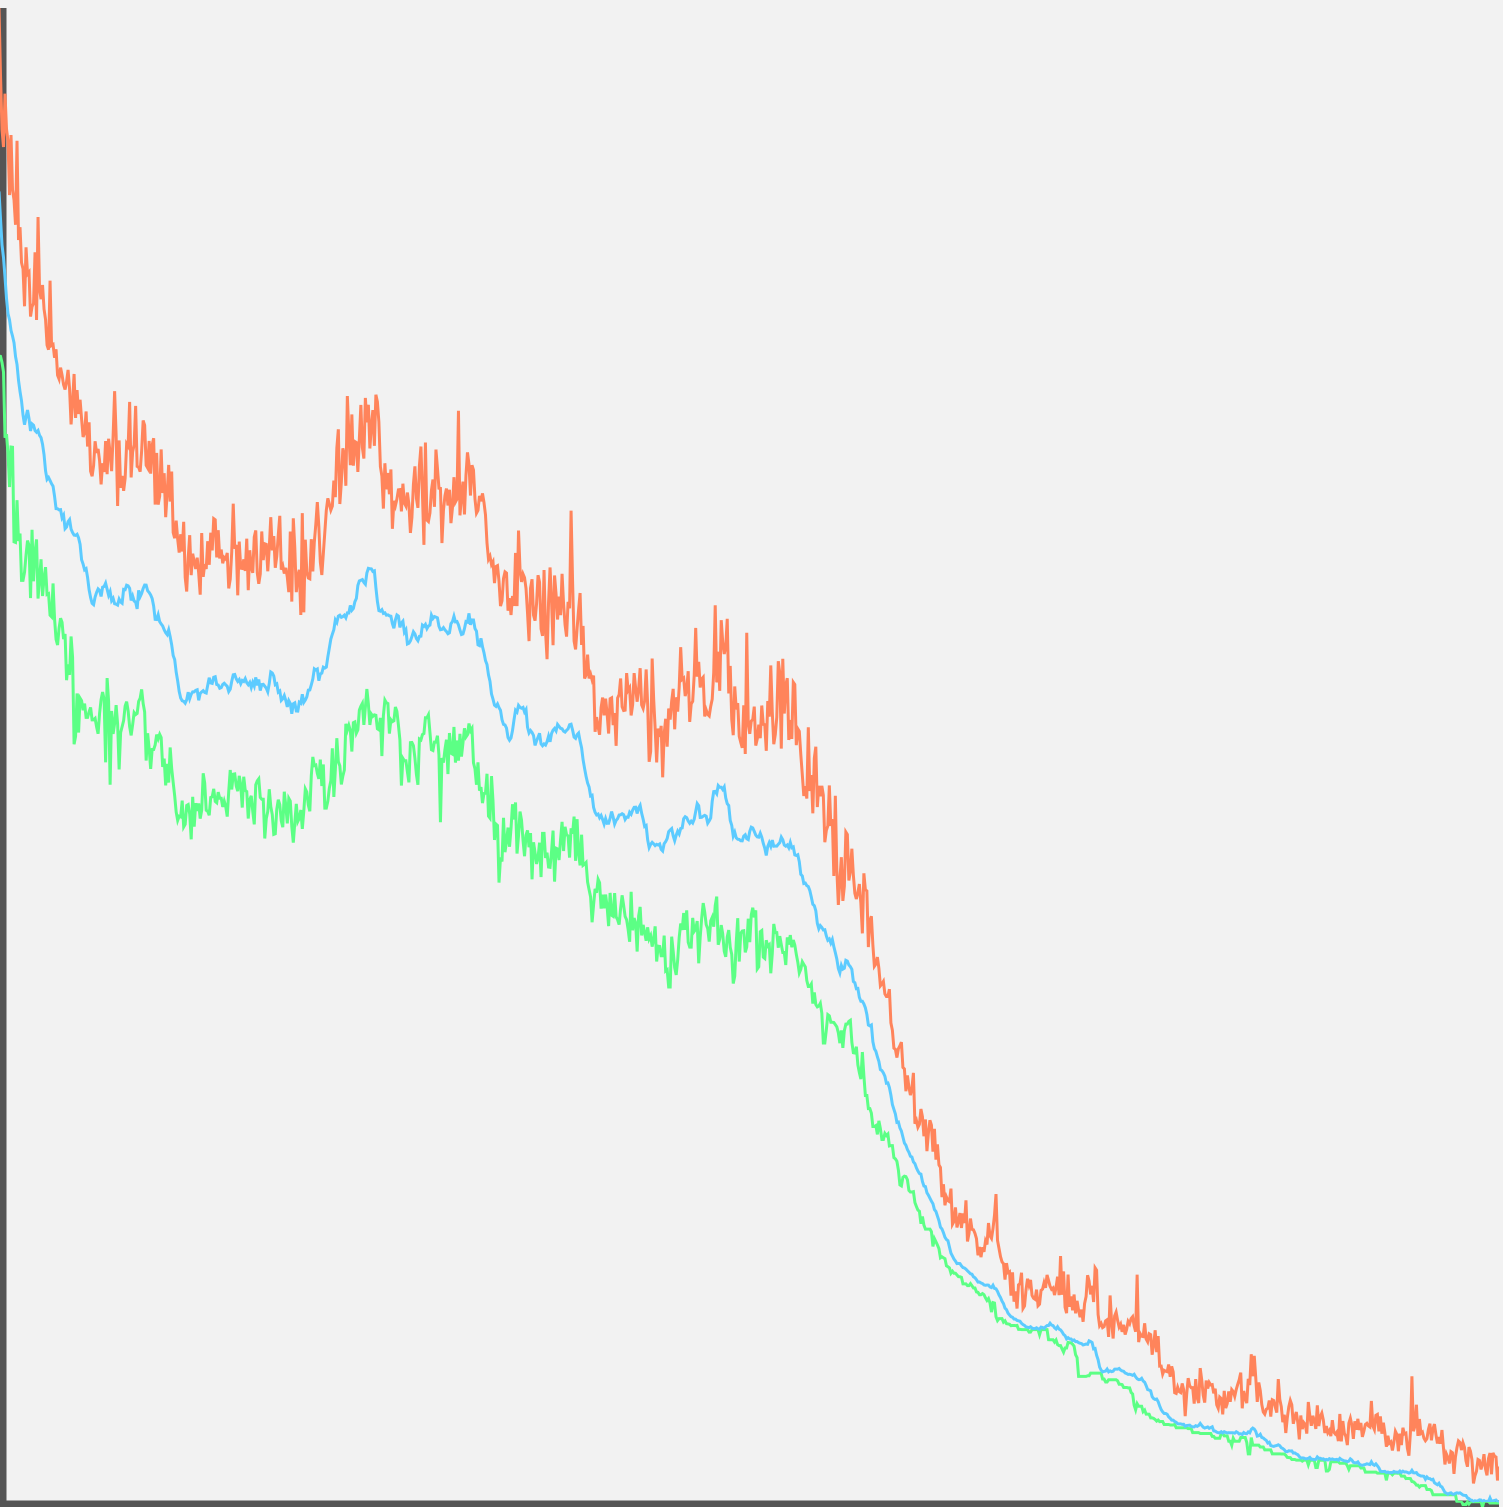
\includegraphics[width=0.45\textwidth]{tour-0-quality-1000}} &
	\FramePic{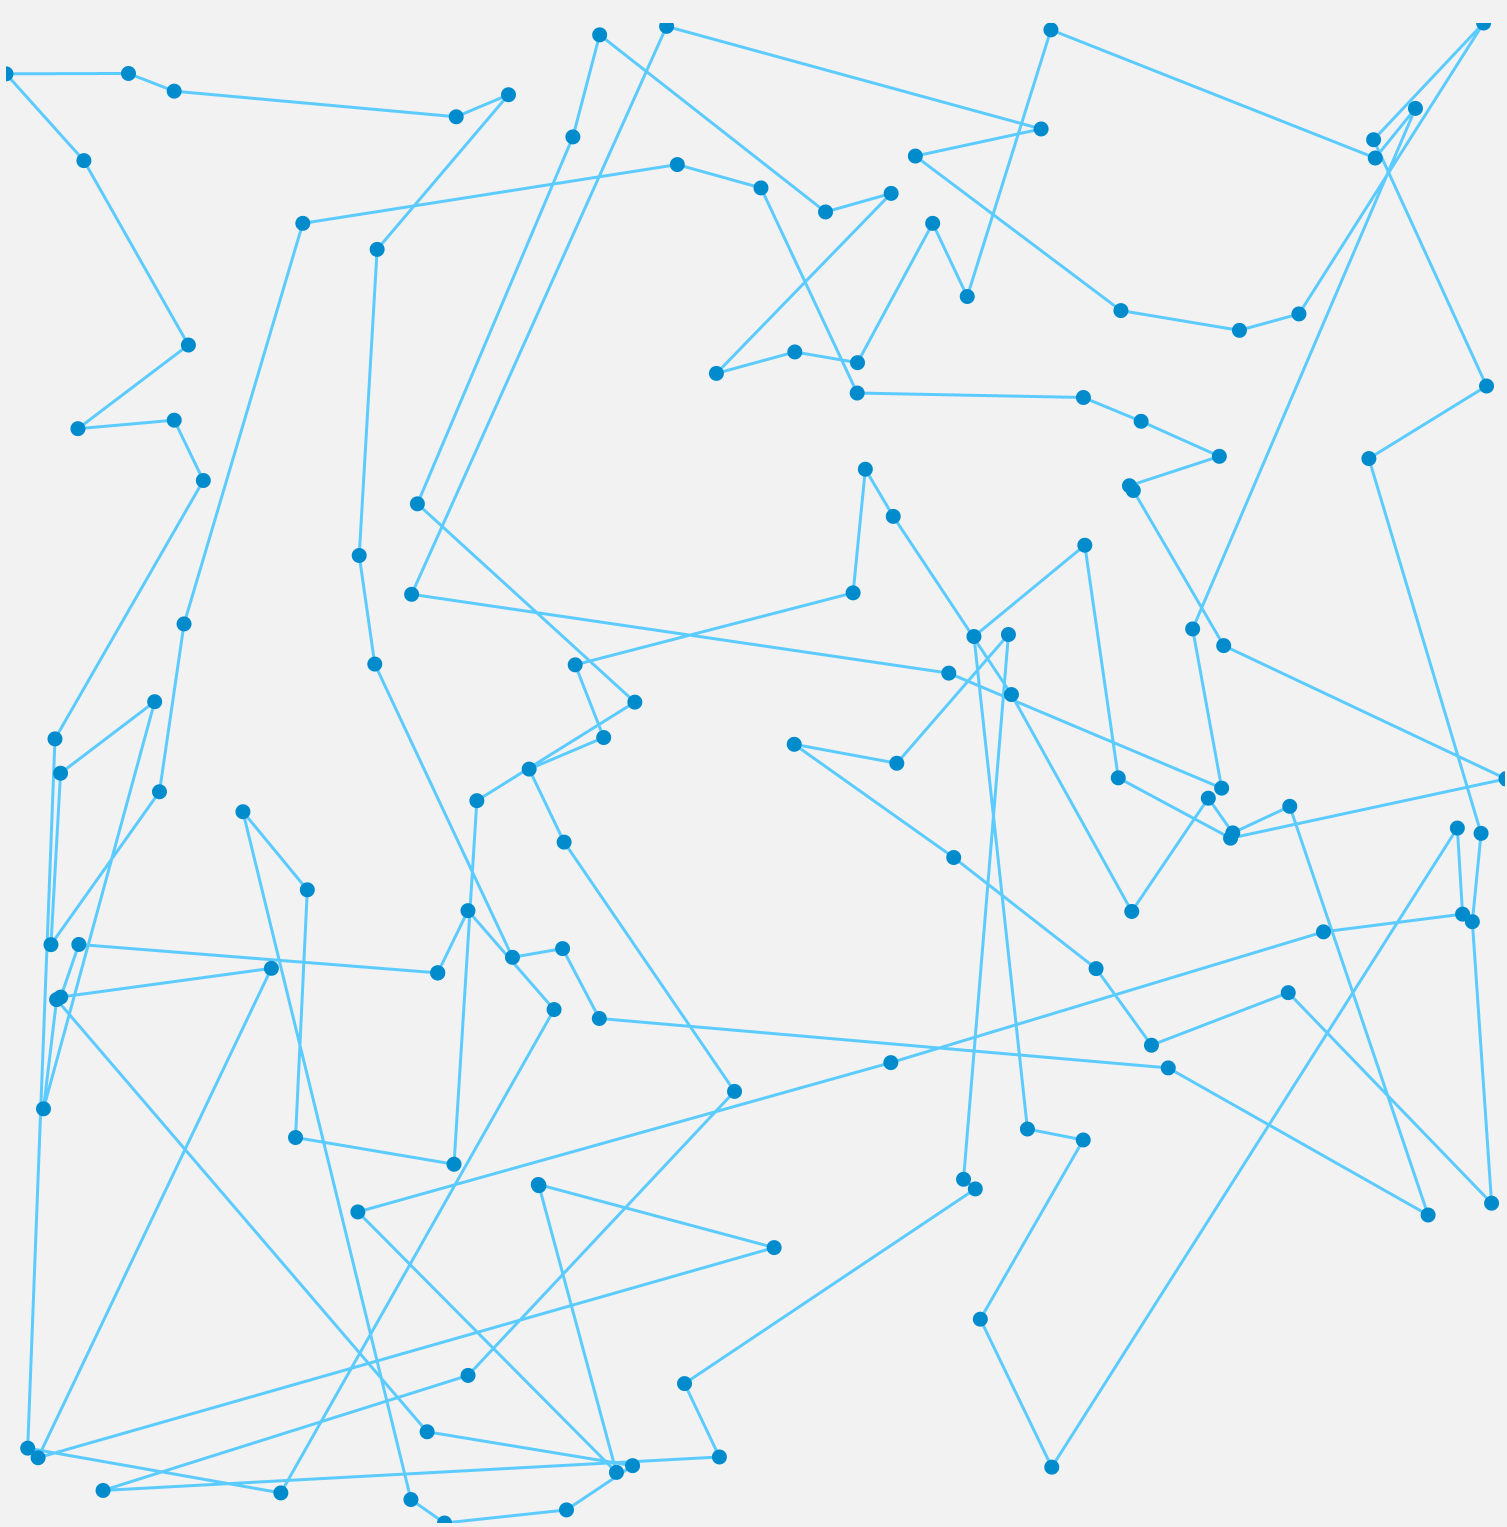
\includegraphics[width=0.45\textwidth]{tour-0-1000}} \\
	(a) & (b) \\
	\FramePic{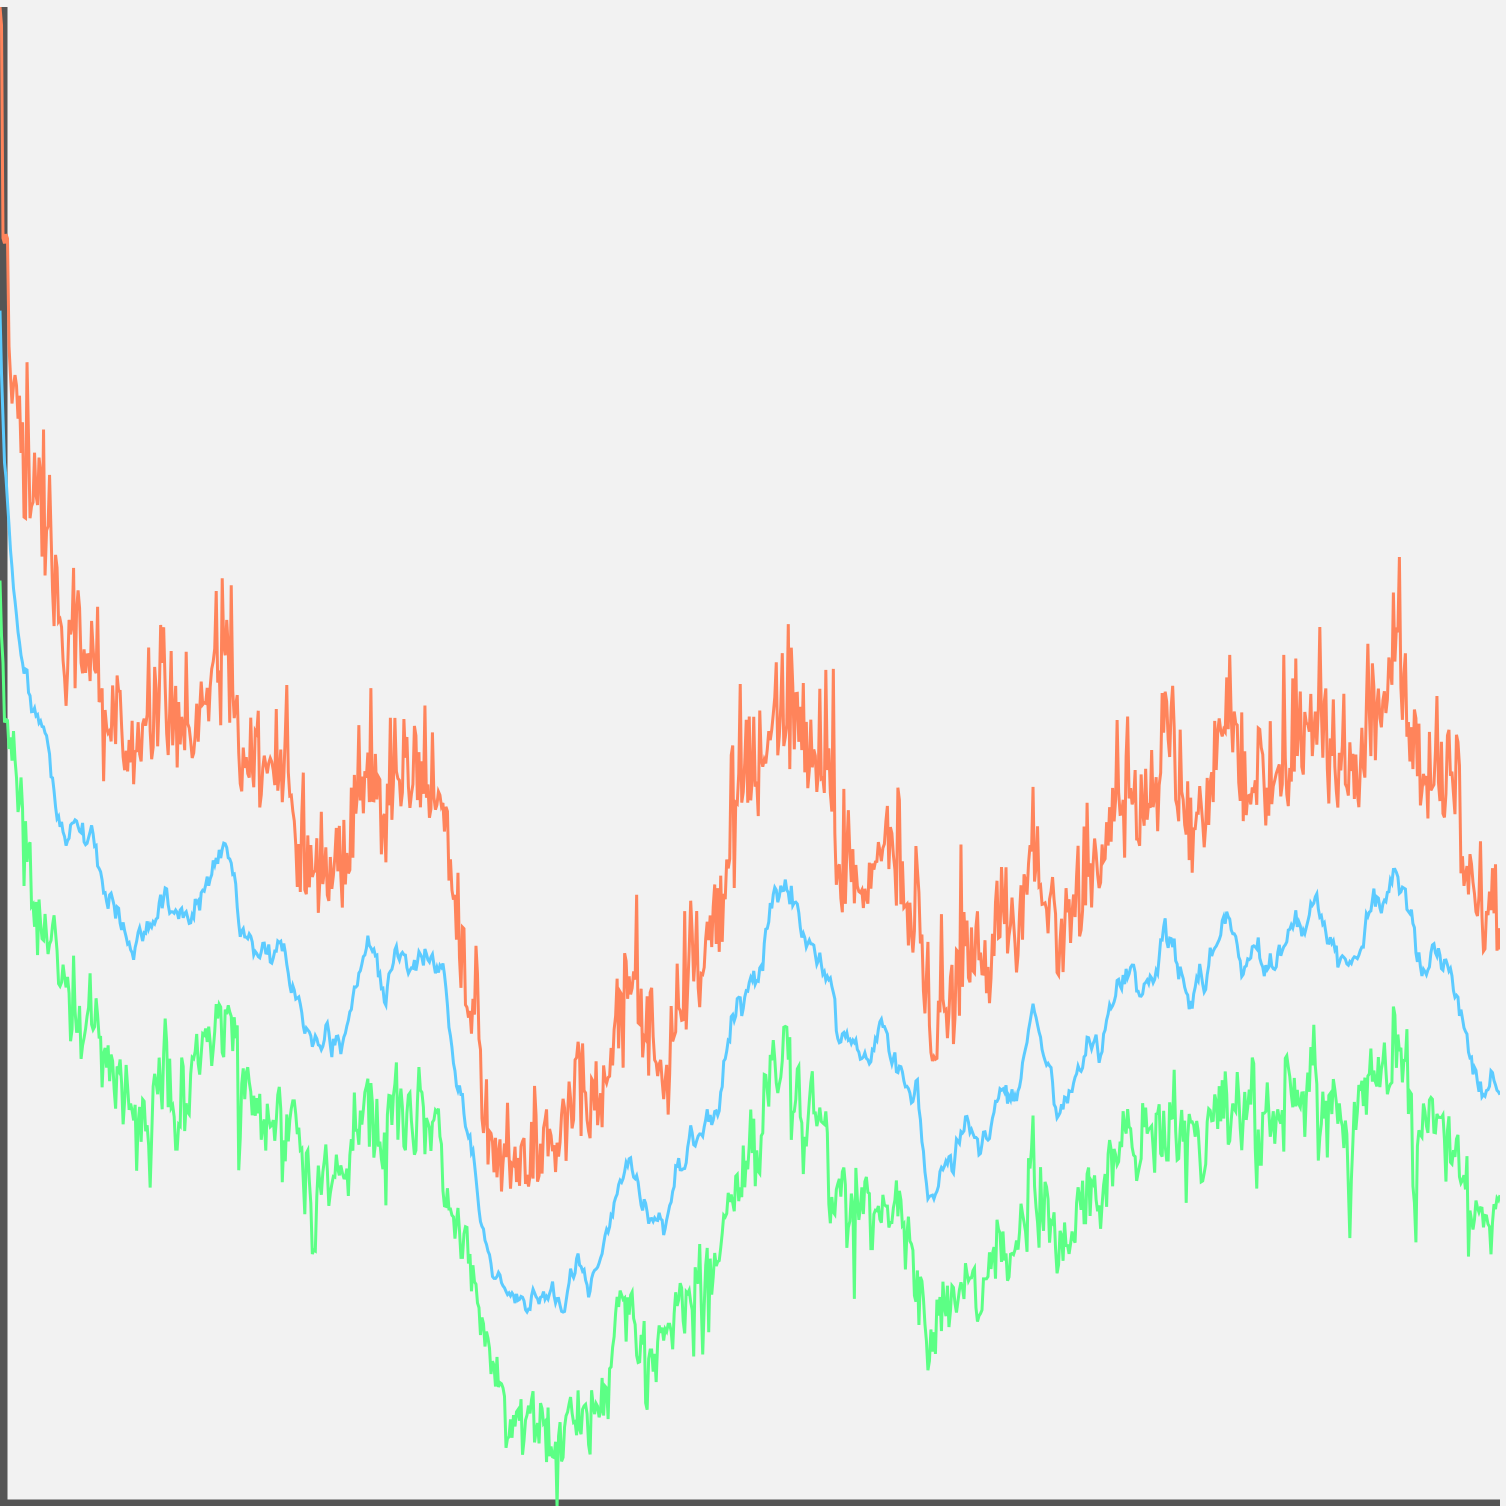
\includegraphics[width=0.45\textwidth]{tour-1-quality-1000}} &
	\FramePic{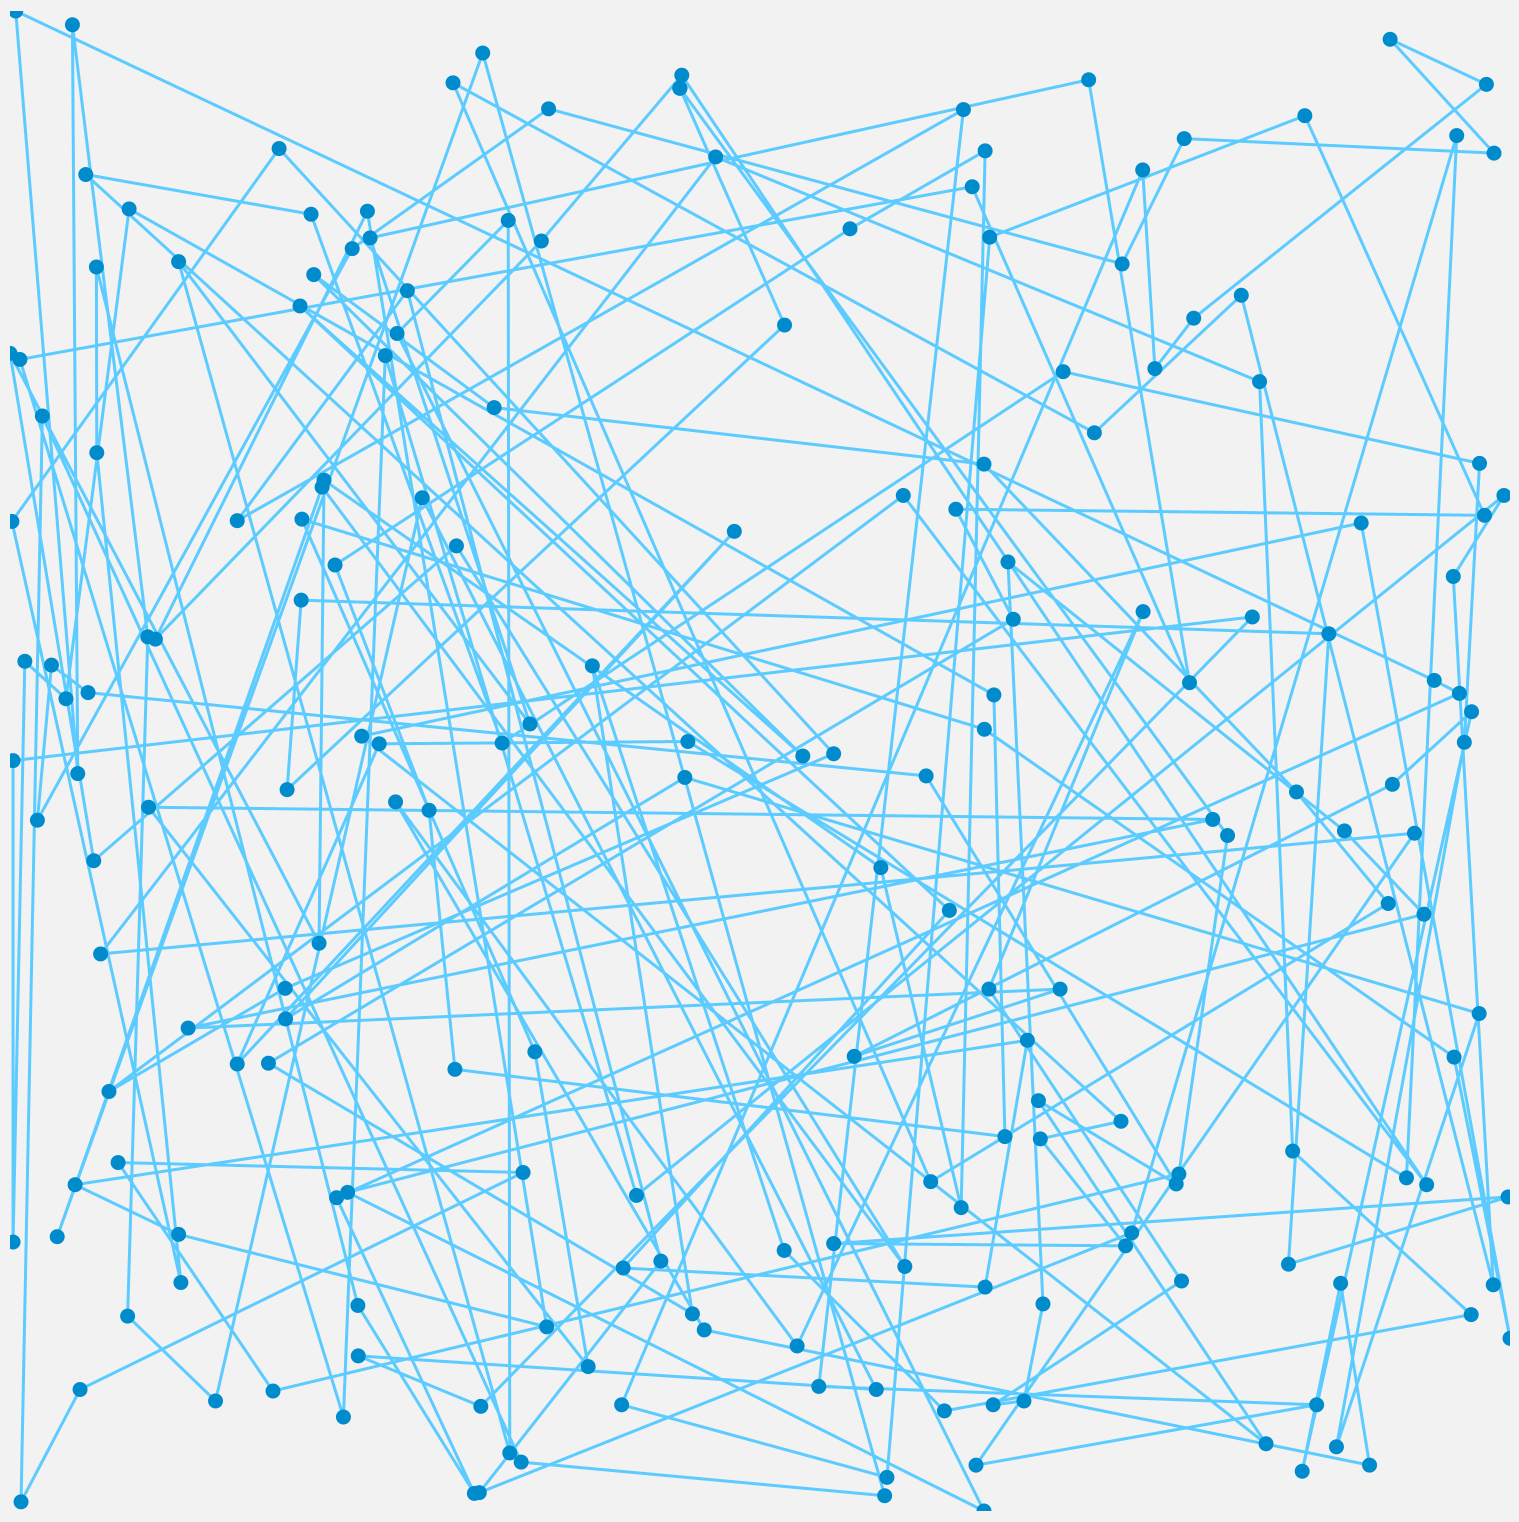
\includegraphics[width=0.45\textwidth]{tour-1-1000}} \\
	(c) & (d)
\end{tabular}
\caption{Ergebnisse bei 1000 Iterationen: 'ch130' Qualitätsverlauf~(a); 'ch130' beste Tour~(b); 'kroA200' Qualitätsverlauf~(c) 'kroA200' beste Tour~(d).}
\label{fig:tour-x-1000}
\end{figure}

\begin{figure}[h]
\centering\small
\begin{tabular}{cc}
	\FramePic{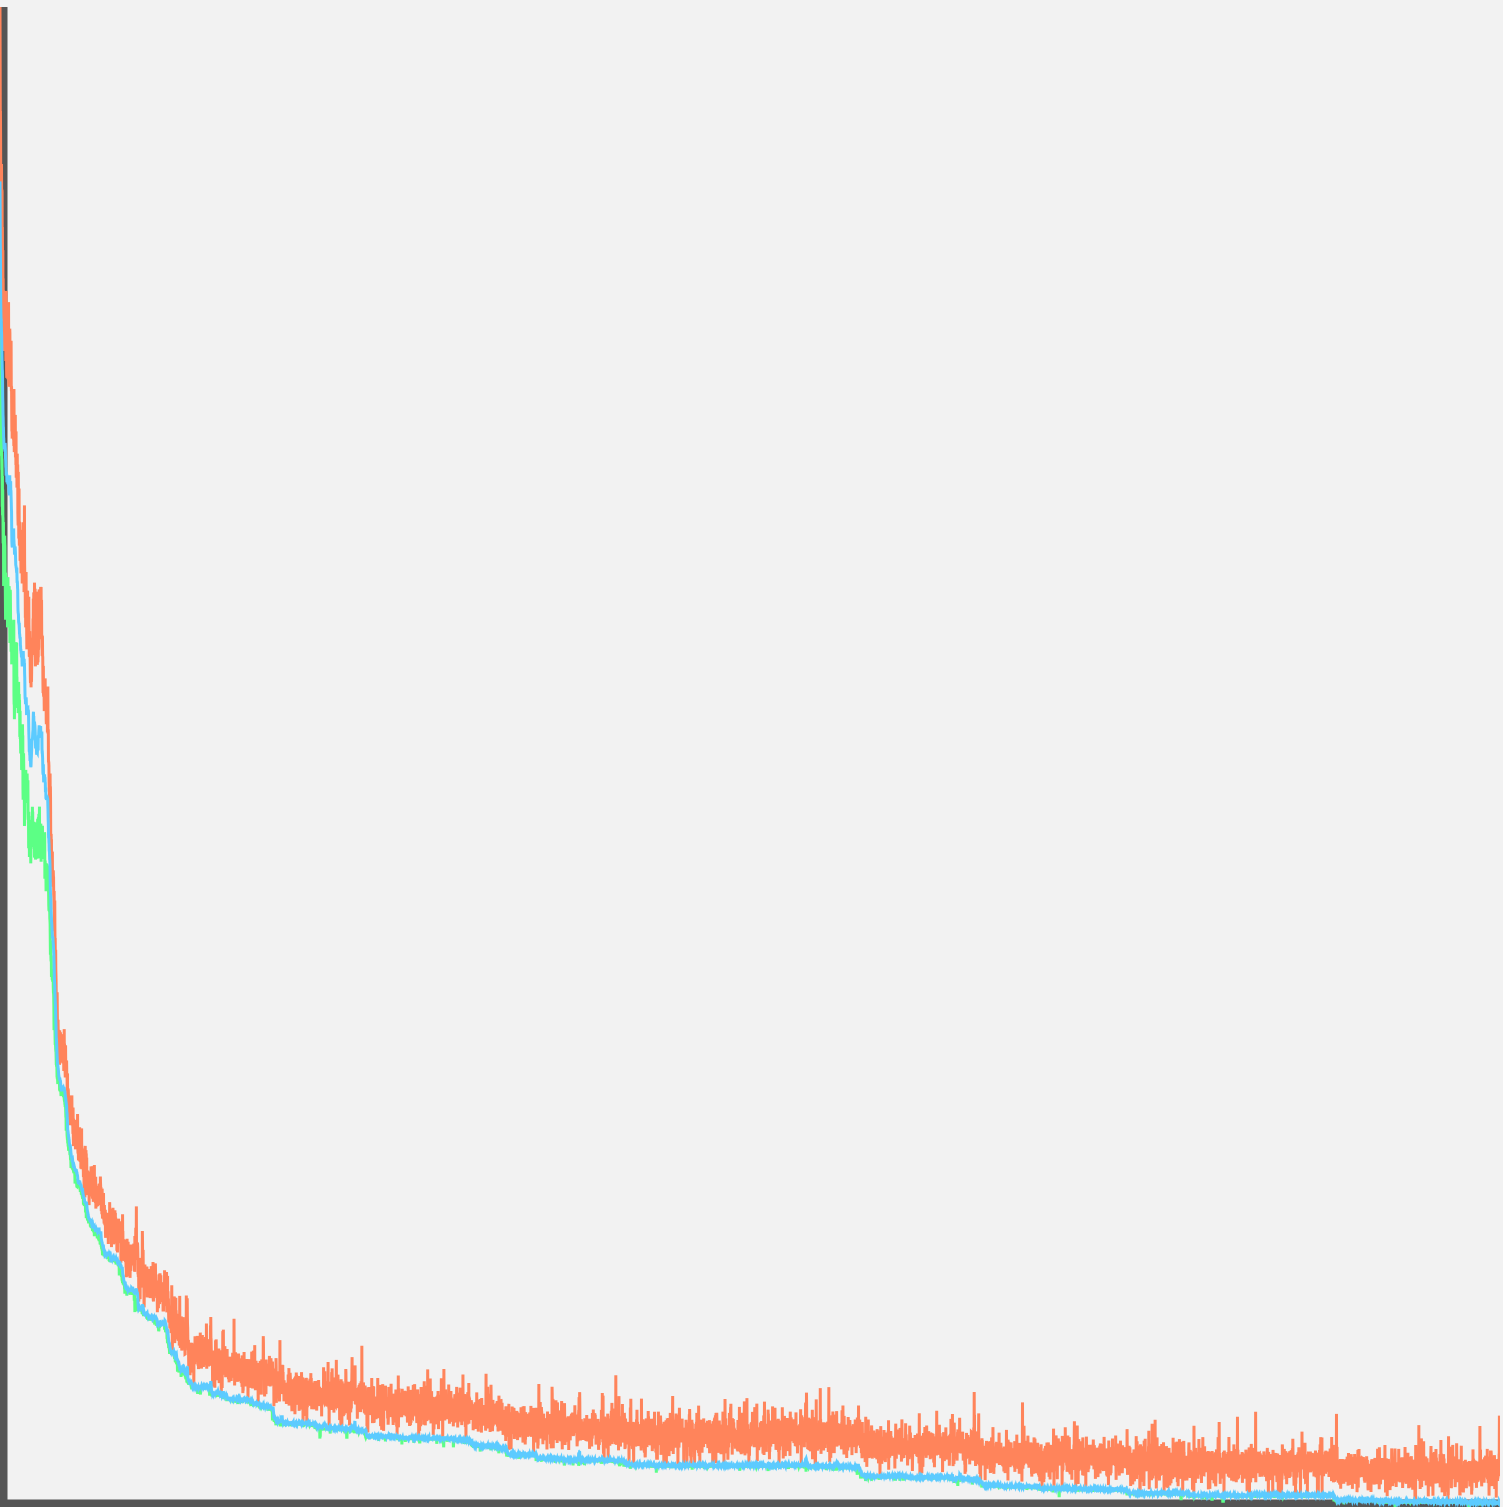
\includegraphics[width=0.45\textwidth]{tour-0-quality-10'000}} &
	\FramePic{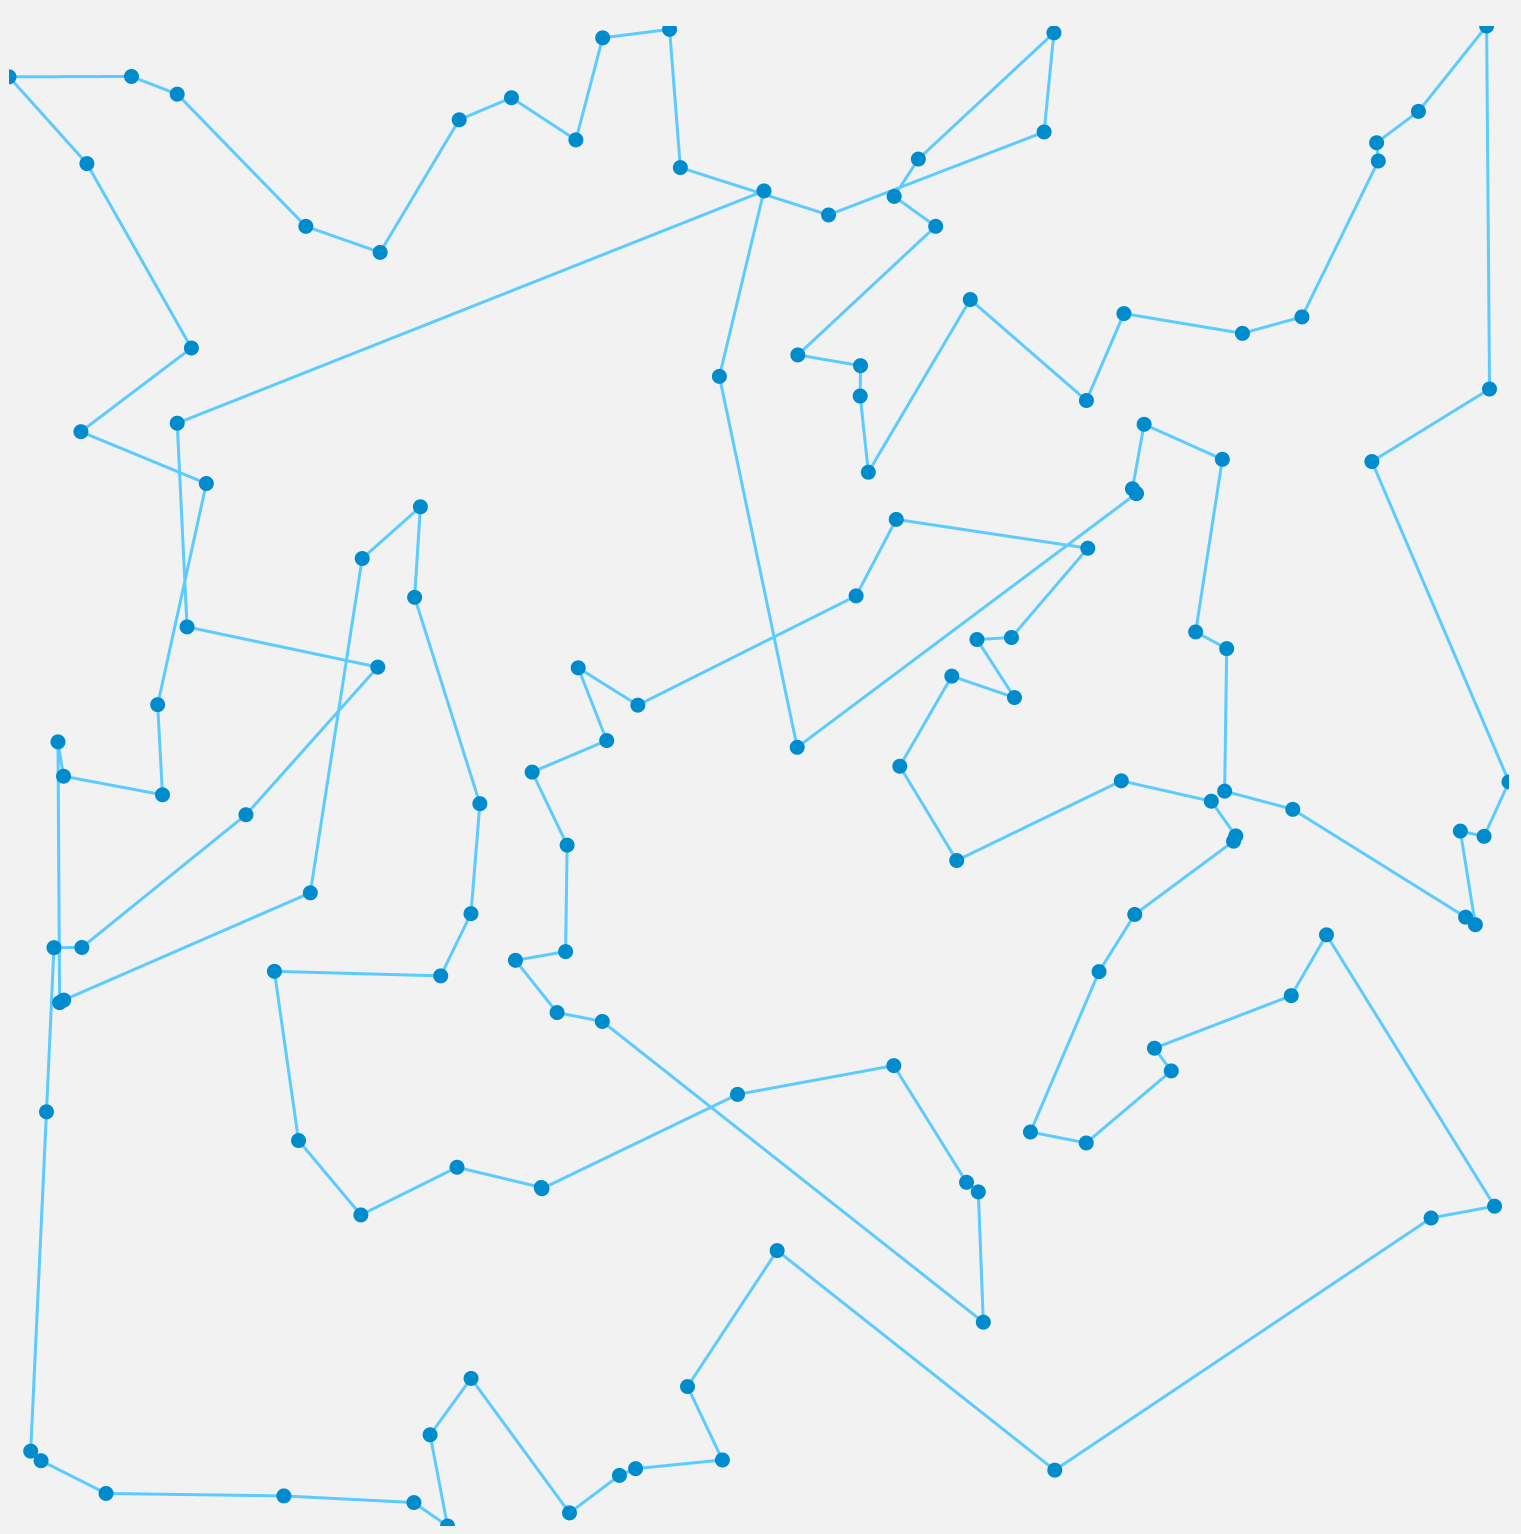
\includegraphics[width=0.45\textwidth]{tour-0-10'000}} \\
	(a) & (b) \\
	\FramePic{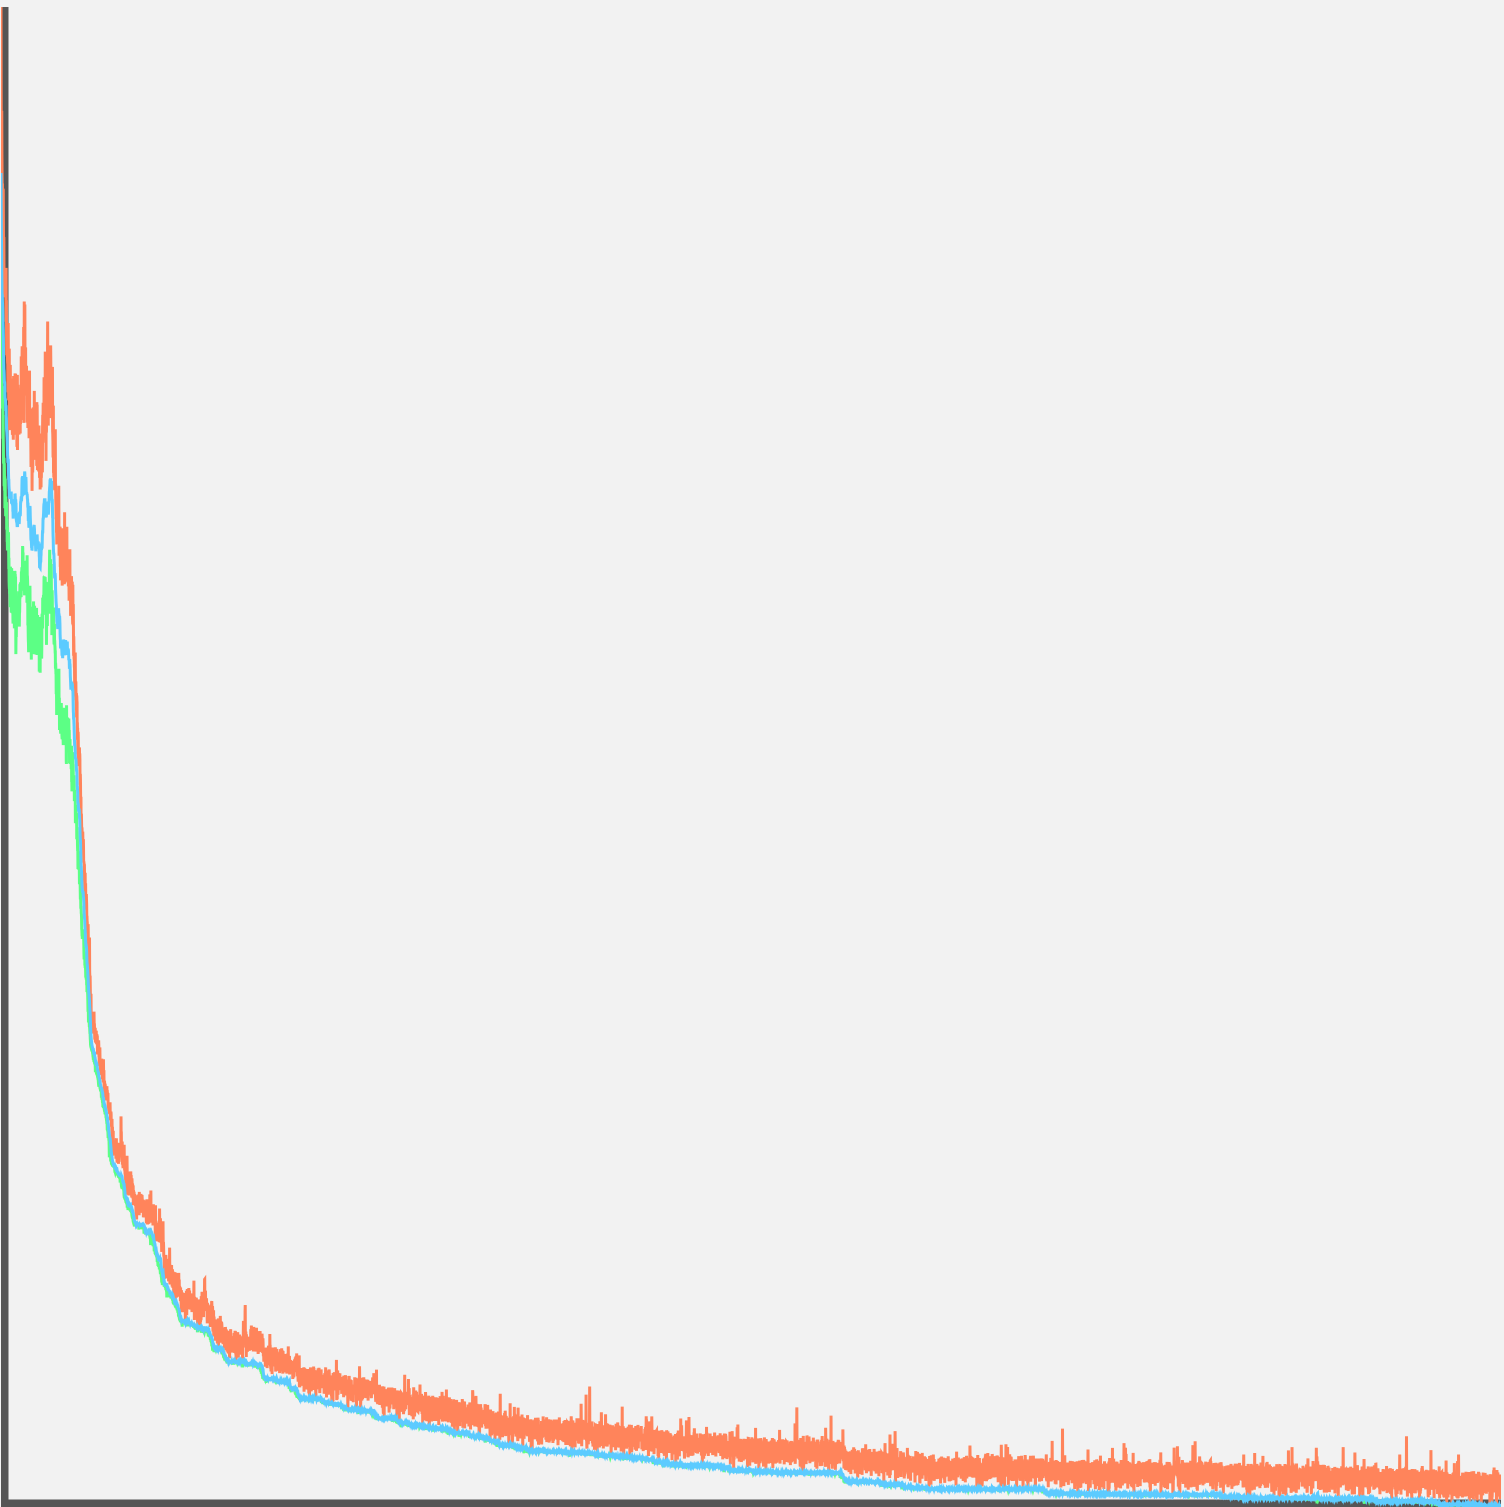
\includegraphics[width=0.45\textwidth]{tour-1-quality-10'000}} &
	\FramePic{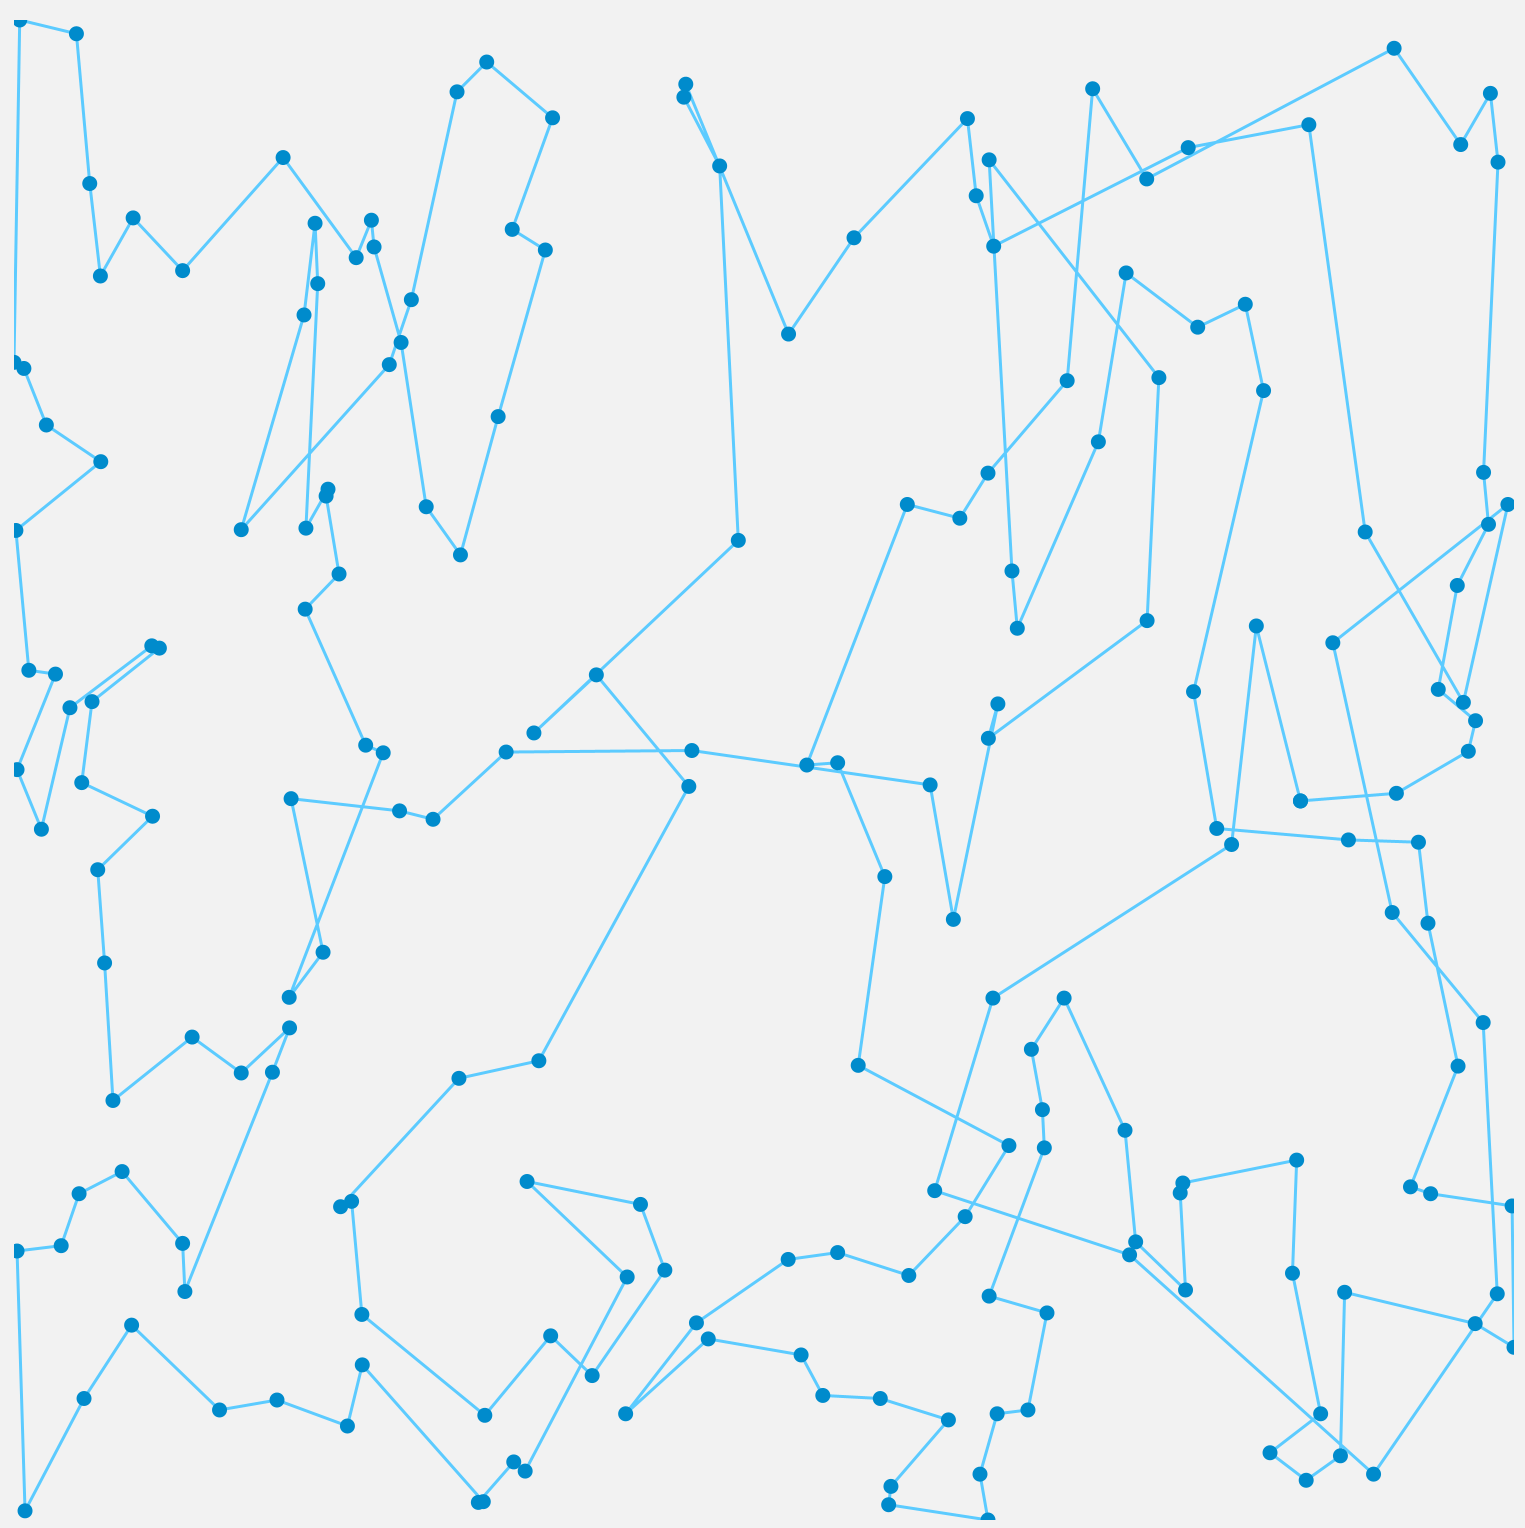
\includegraphics[width=0.45\textwidth]{tour-1-10'000}} \\
	(c) & (d)
\end{tabular}
\caption{Ergebnisse bei 10000 Iterationen: 'ch130' Qualitätsverlauf~(a); 'ch130' beste Tour~(b); 'kroA200' Qualitätsverlauf~(c) 'kroA200' beste Tour~(d).}
\label{fig:tour-x-10000}
\end{figure}

\begin{figure}[h]
\centering\small
\begin{tabular}{cc}
	\FramePic{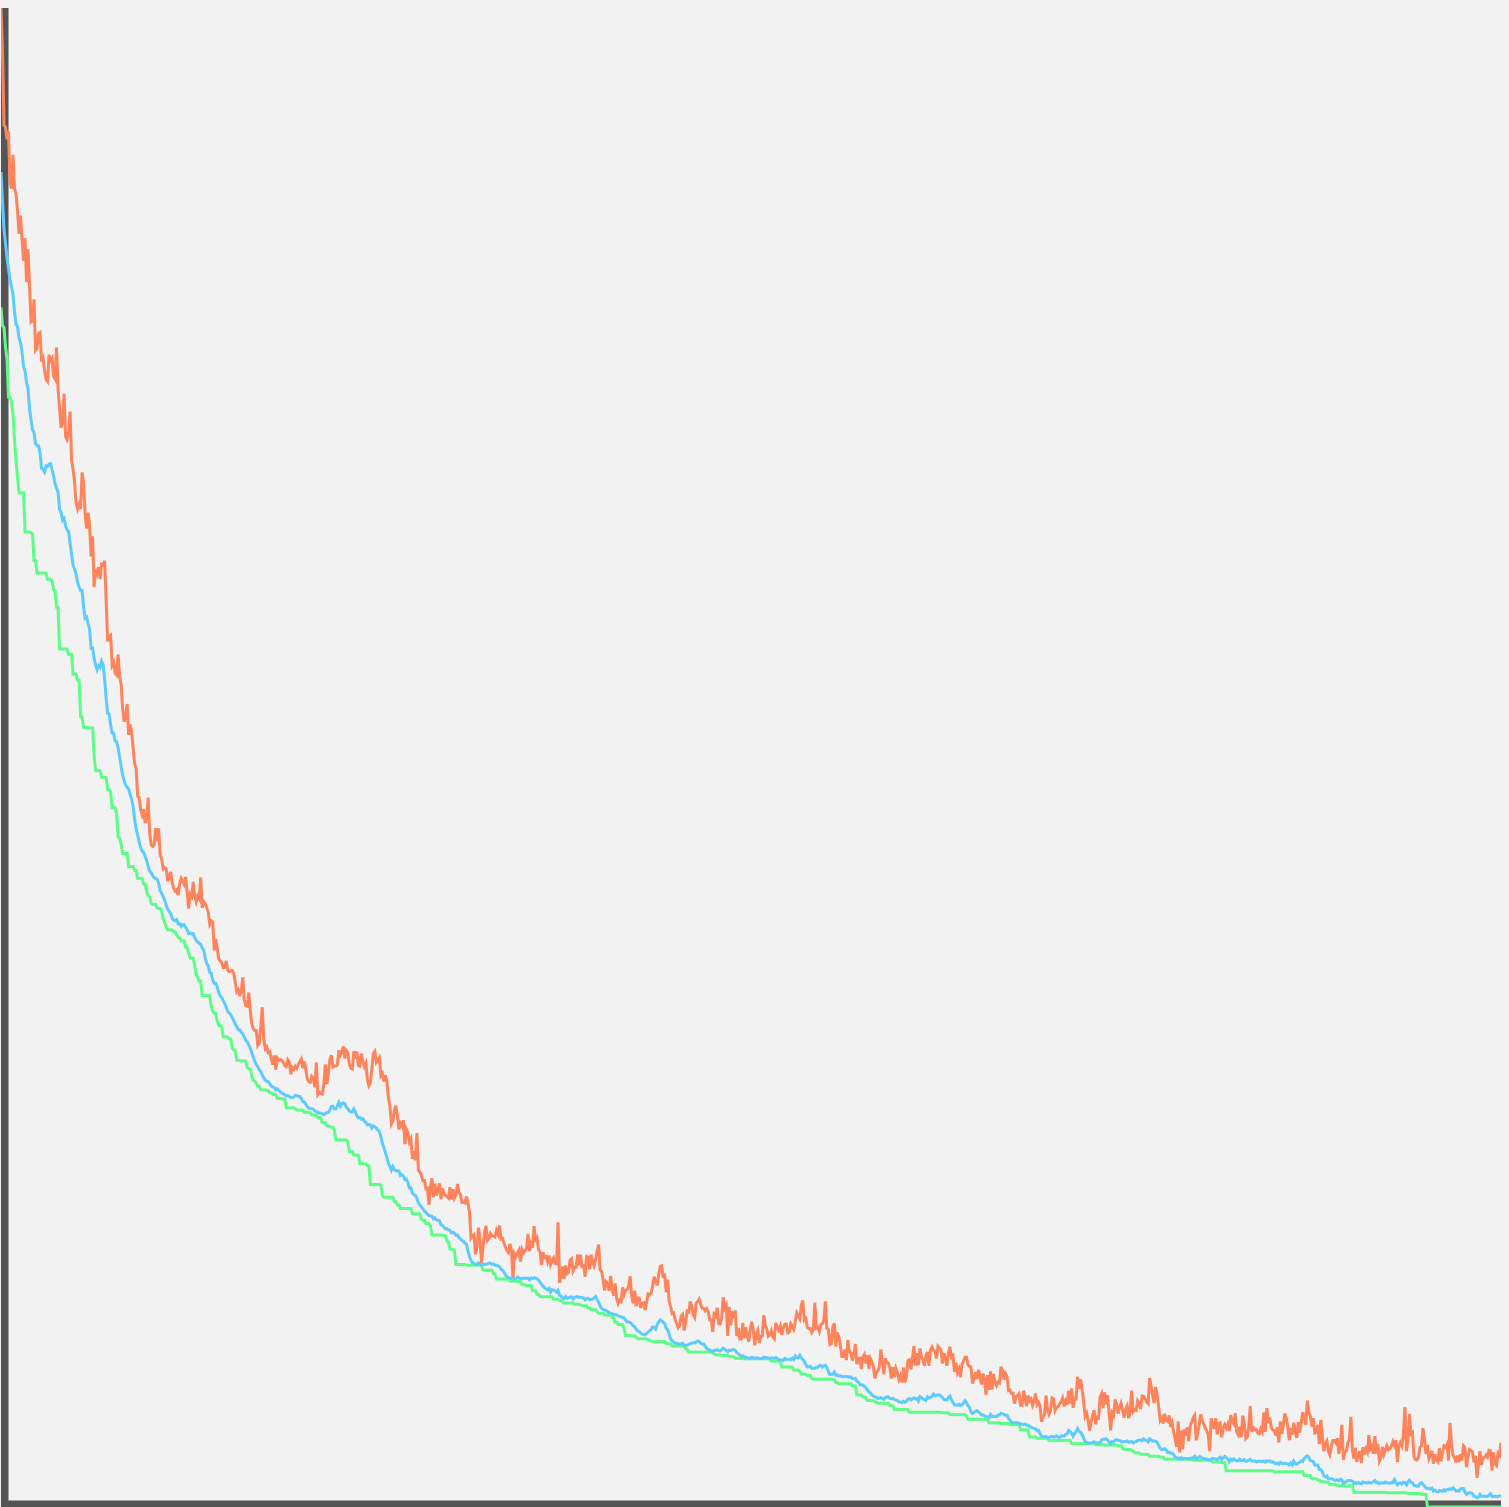
\includegraphics[width=0.45\textwidth]{tour-0-elite-quality-1000}} &
	\FramePic{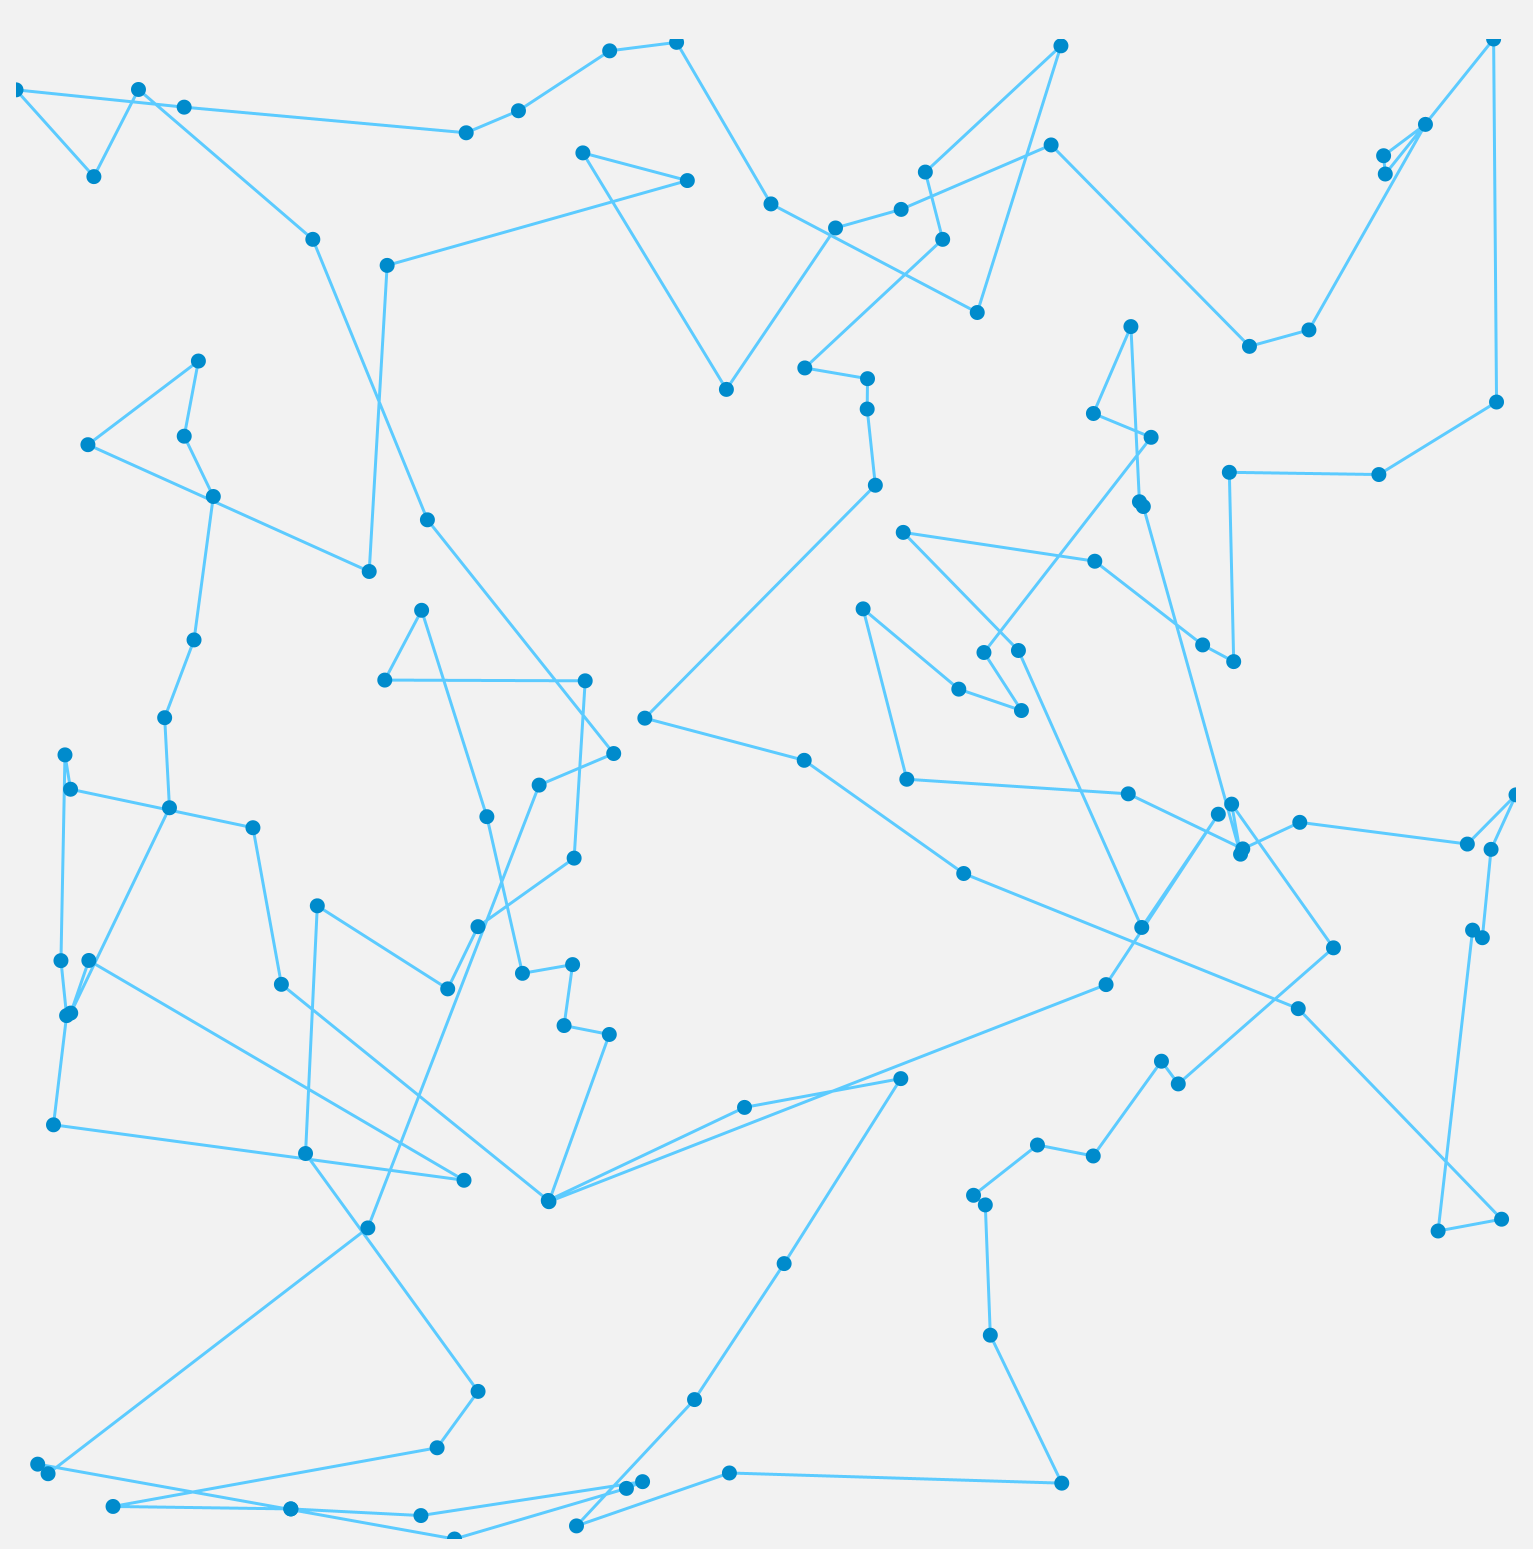
\includegraphics[width=0.45\textwidth]{tour-0-elite-1000}} \\
	(a) & (b) \\
	\FramePic{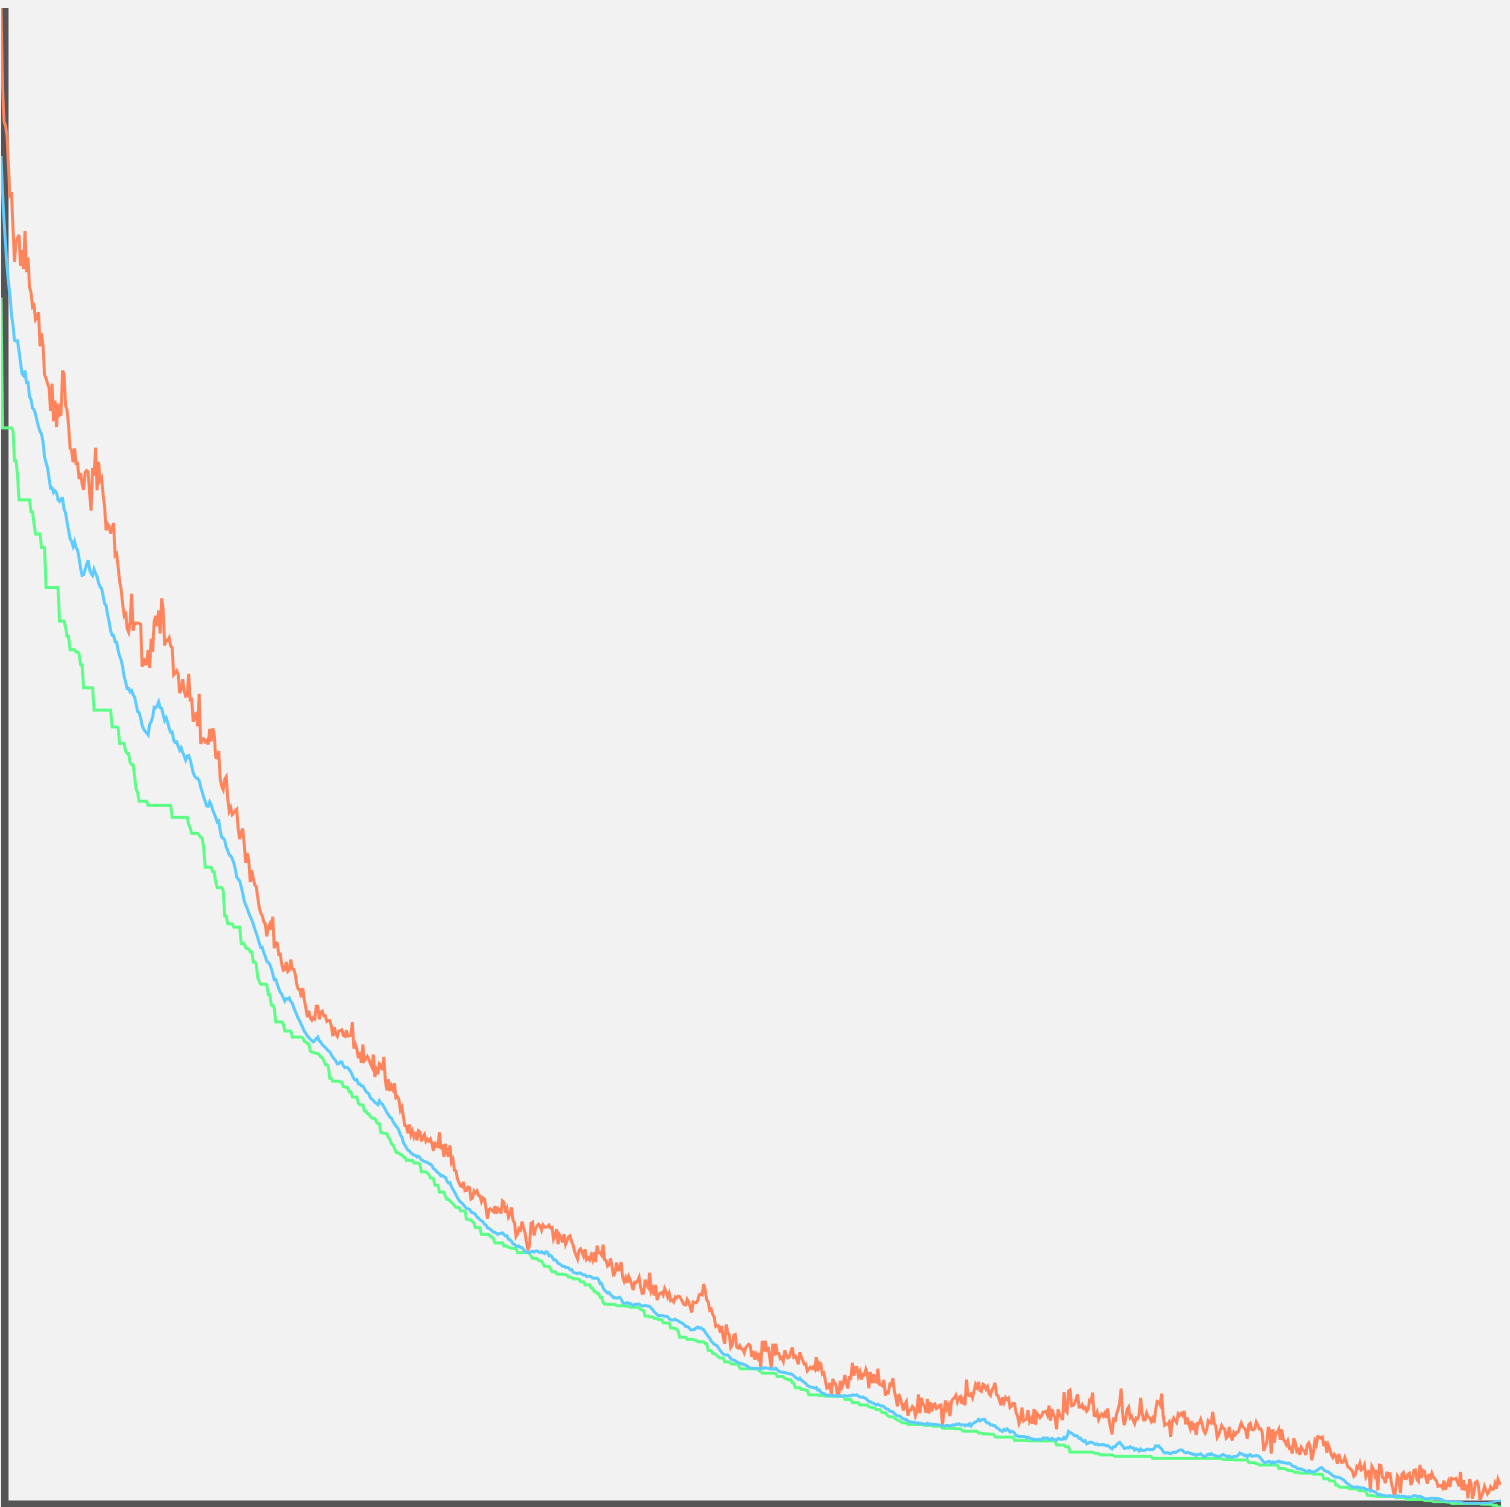
\includegraphics[width=0.45\textwidth]{tour-1-elite-quality-1000}} &
	\FramePic{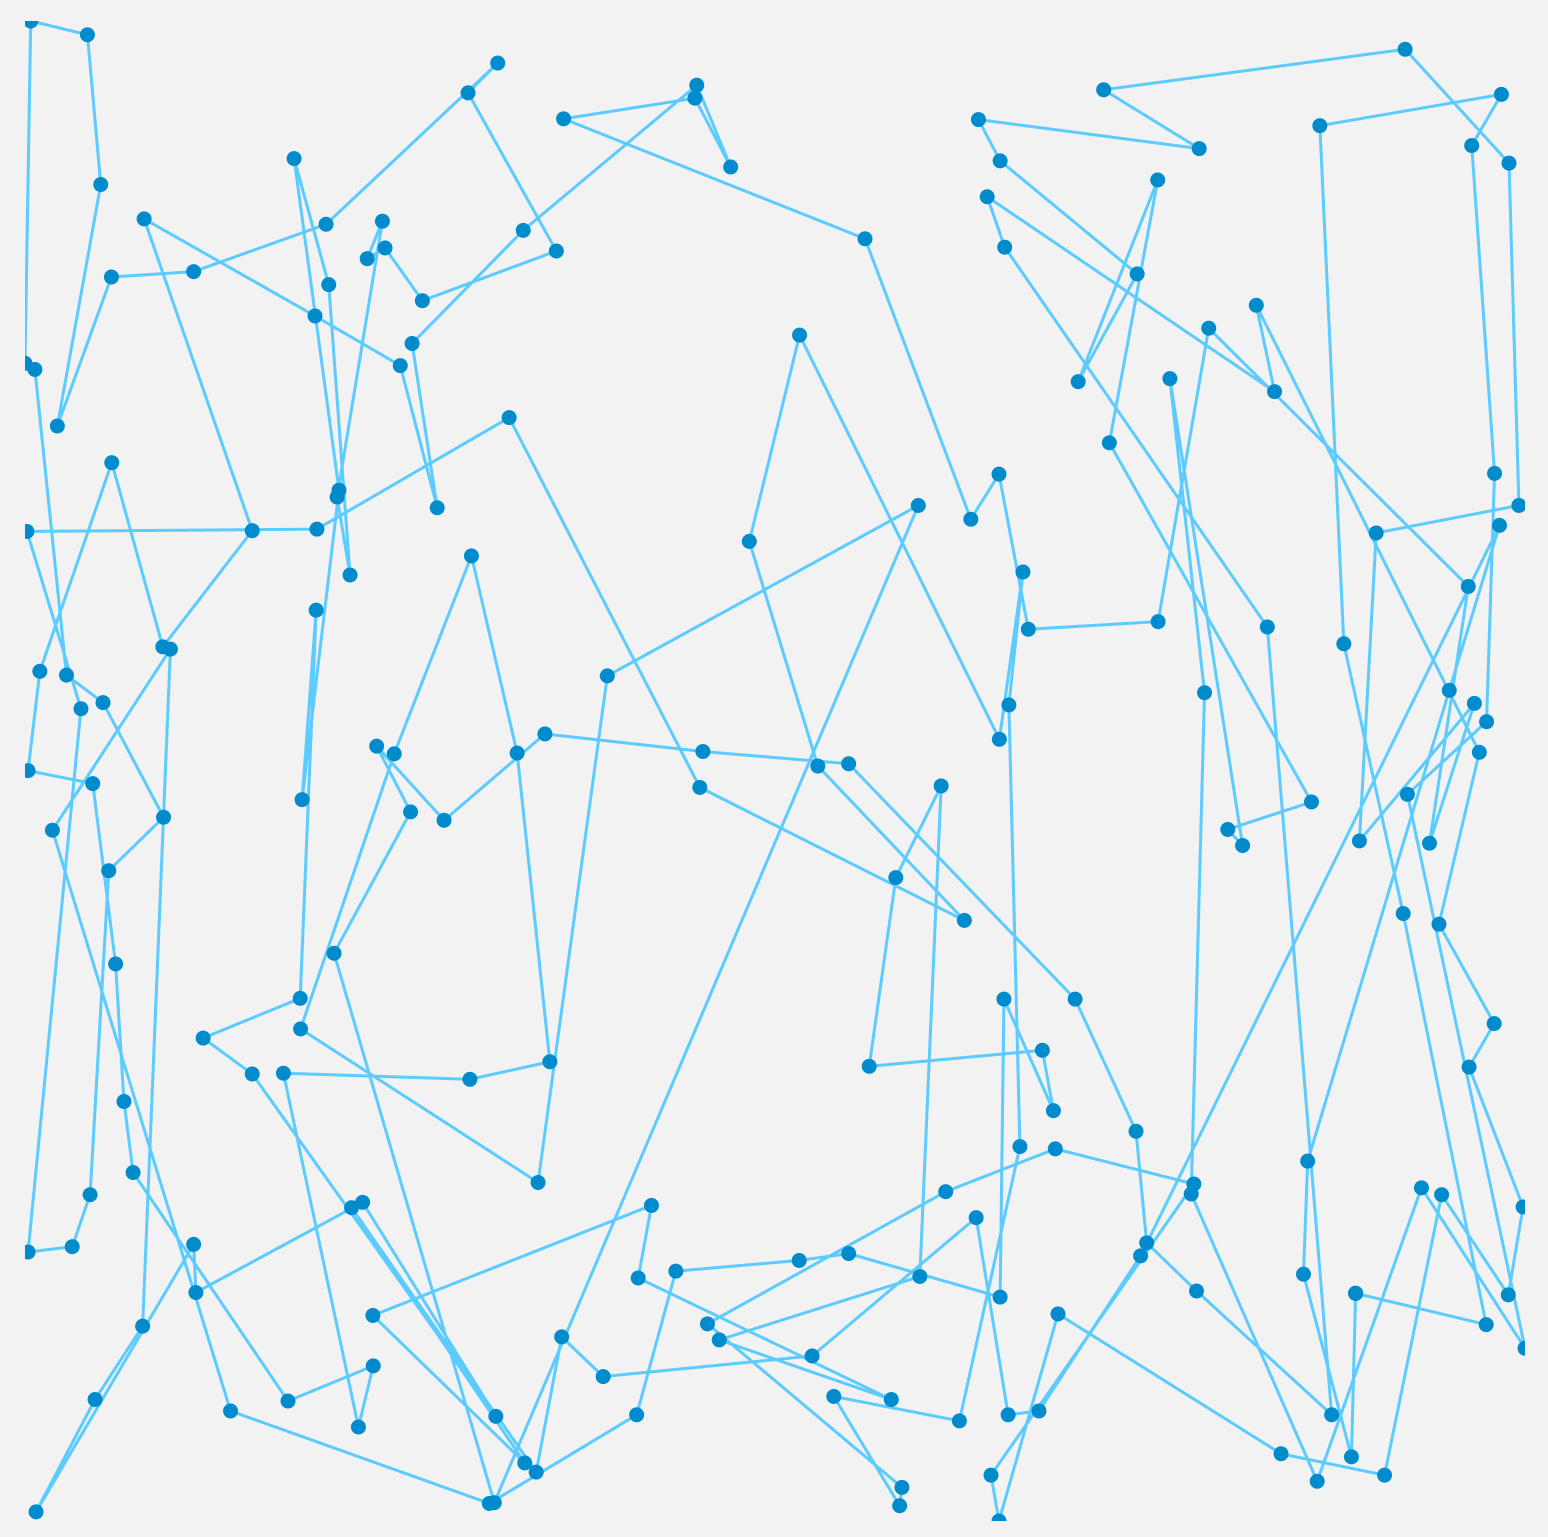
\includegraphics[width=0.45\textwidth]{tour-1-elite-1000}} \\
	(c) & (d)
\end{tabular}
\caption{Ergebnisse bei 1000 Iterationen; \texttt{1-elitism} aktiviert : 'ch130' Qualitätsverlauf~(a); 'ch130' beste Tour~(b); 'kroA200' Qualitätsverlauf~(c) 'kroA200' beste Tour~(d).}
\label{fig:tour-x-elite-1000}
\end{figure}

%----------------------------------------------------------------------------------------------------------------
\clearpage
\subsubsection{Beste Tour}

\begin{figure}[h]
\centering
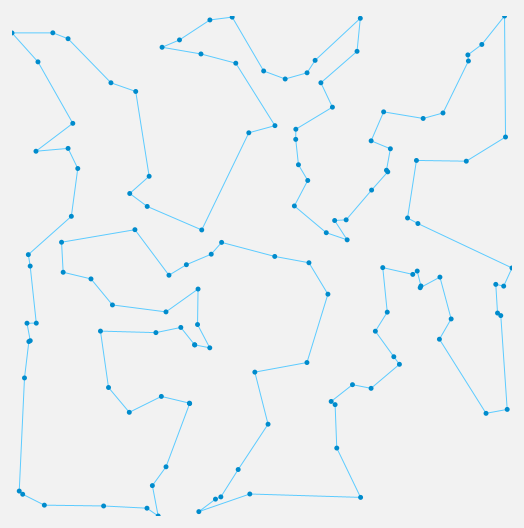
\includegraphics[width=.55\textwidth]{tour-0-1'000'000}
\caption{Beste tour für 'ch130' nach 1000000 Iterationen.}
\label{fig:ch130-1000000}
\end{figure}

\begin{figure}[h]
\centering
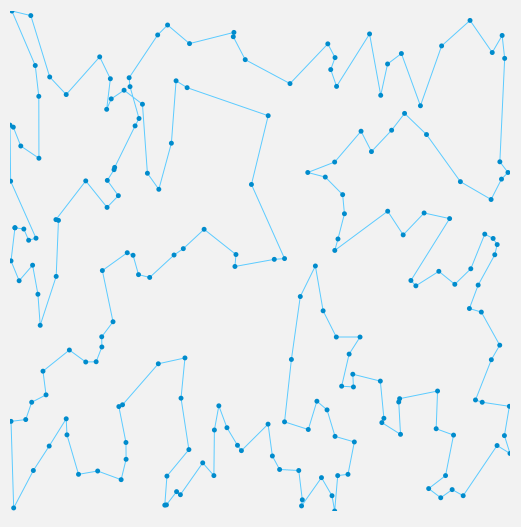
\includegraphics[width=.55\textwidth]{tour-1-1'000'000}
\caption{Beste tour für 'kroA200' nach 1000000 Iterationen.}
\label{fig:kroA200-1000000}
\end{figure}

%%%-----------------------------------------------------------------------------

%\section*{Zusammenfassung und Anmerkungen}

%%%-----------------------------------------------------------------------------

% \section*{Quellen}

% \printbibliography[heading=noheader]

%%%-----------------------------------------------------------------------------
\end{document}
%%%-----------------------------------------------------------------------------